\documentclass[twoside]{book}

% Packages required by doxygen
\usepackage{fixltx2e}
\usepackage{calc}
\usepackage{doxygen}
\usepackage[export]{adjustbox} % also loads graphicx
\usepackage{graphicx}
\usepackage[utf8]{inputenc}
\usepackage{makeidx}
\usepackage{multicol}
\usepackage{multirow}
\PassOptionsToPackage{warn}{textcomp}
\usepackage{textcomp}
\usepackage[nointegrals]{wasysym}
\usepackage[table]{xcolor}

% Font selection
\usepackage[T1]{fontenc}
\usepackage[scaled=.90]{helvet}
\usepackage{courier}
\usepackage{amssymb}
\usepackage{sectsty}
\renewcommand{\familydefault}{\sfdefault}
\allsectionsfont{%
  \fontseries{bc}\selectfont%
  \color{darkgray}%
}
\renewcommand{\DoxyLabelFont}{%
  \fontseries{bc}\selectfont%
  \color{darkgray}%
}
\newcommand{\+}{\discretionary{\mbox{\scriptsize$\hookleftarrow$}}{}{}}

% Page & text layout
\usepackage{geometry}
\geometry{%
  a4paper,%
  top=2.5cm,%
  bottom=2.5cm,%
  left=2.5cm,%
  right=2.5cm%
}
\tolerance=750
\hfuzz=15pt
\hbadness=750
\setlength{\emergencystretch}{15pt}
\setlength{\parindent}{0cm}
\setlength{\parskip}{3ex plus 2ex minus 2ex}
\makeatletter
\renewcommand{\paragraph}{%
  \@startsection{paragraph}{4}{0ex}{-1.0ex}{1.0ex}{%
    \normalfont\normalsize\bfseries\SS@parafont%
  }%
}
\renewcommand{\subparagraph}{%
  \@startsection{subparagraph}{5}{0ex}{-1.0ex}{1.0ex}{%
    \normalfont\normalsize\bfseries\SS@subparafont%
  }%
}
\makeatother

% Headers & footers
\usepackage{fancyhdr}
\pagestyle{fancyplain}
\fancyhead[LE]{\fancyplain{}{\bfseries\thepage}}
\fancyhead[CE]{\fancyplain{}{}}
\fancyhead[RE]{\fancyplain{}{\bfseries\leftmark}}
\fancyhead[LO]{\fancyplain{}{\bfseries\rightmark}}
\fancyhead[CO]{\fancyplain{}{}}
\fancyhead[RO]{\fancyplain{}{\bfseries\thepage}}
\fancyfoot[LE]{\fancyplain{}{}}
\fancyfoot[CE]{\fancyplain{}{}}
\fancyfoot[RE]{\fancyplain{}{\bfseries\scriptsize Generated by Doxygen }}
\fancyfoot[LO]{\fancyplain{}{\bfseries\scriptsize Generated by Doxygen }}
\fancyfoot[CO]{\fancyplain{}{}}
\fancyfoot[RO]{\fancyplain{}{}}
\renewcommand{\footrulewidth}{0.4pt}
\renewcommand{\chaptermark}[1]{%
  \markboth{#1}{}%
}
\renewcommand{\sectionmark}[1]{%
  \markright{\thesection\ #1}%
}

% Indices & bibliography
\usepackage{natbib}
\usepackage[titles]{tocloft}
\setcounter{tocdepth}{3}
\setcounter{secnumdepth}{5}
\makeindex

% Hyperlinks (required, but should be loaded last)
\usepackage{ifpdf}
\ifpdf
  \usepackage[pdftex,pagebackref=true]{hyperref}
\else
  \usepackage[ps2pdf,pagebackref=true]{hyperref}
\fi
\hypersetup{%
  colorlinks=true,%
  linkcolor=blue,%
  citecolor=blue,%
  unicode%
}

% Custom commands
\newcommand{\clearemptydoublepage}{%
  \newpage{\pagestyle{empty}\cleardoublepage}%
}

\usepackage{caption}
\captionsetup{labelsep=space,justification=centering,font={bf},singlelinecheck=off,skip=4pt,position=top}

%===== C O N T E N T S =====

\begin{document}

% Titlepage & ToC
\hypersetup{pageanchor=false,
             bookmarksnumbered=true,
             pdfencoding=unicode
            }
\pagenumbering{alph}
\begin{titlepage}
\vspace*{7cm}
\begin{center}%
{\Large Assessment\+Three\+PartB \\[1ex]\large 1.\+0 }\\
\vspace*{1cm}
{\large Generated by Doxygen 1.8.13}\\
\end{center}
\end{titlepage}
\clearemptydoublepage
\pagenumbering{roman}
\tableofcontents
\clearemptydoublepage
\pagenumbering{arabic}
\hypersetup{pageanchor=true}

%--- Begin generated contents ---
\chapter{Assessment Three Part B I\+PC Socket Application}
\label{index}\hypertarget{index}{}\hypertarget{index_author_sec}{}\section{Author}\label{index_author_sec}
Author\+: Mark Schafers\hypertarget{index_reference_sec}{}\section{References}\label{index_reference_sec}
References\+: \href{https://www.youtube.com/channel/UCjEwVWVFkhMRFoSYWXIND6Q}{\tt https\+://www.\+youtube.\+com/channel/\+U\+Cj\+Ew\+V\+W\+V\+Fkh\+M\+R\+Fo\+S\+Y\+W\+X\+I\+N\+D6Q} -\/ Videos\+: C\# Socket Programming -\/ Multiple Clients, C\# Async Sockets Part 1\+: Basics, C\# Async Sockets Part 2\+: Robustness, C\# Async Sockets Part 3\+: Lightweight Packaging\hypertarget{index_description_sec}{}\section{Description}\label{index_description_sec}
This application was designed to demonstrate the use of sockets in I\+PC for assessment three part b of the dynamic data structures unit. A server will accept multiple clients, When a client connects they must first input their name and click send, this will initiate the connection. Once connected a client can enter text and click to send, this will be received on the server end and will be output within the server textbox with the users name displayed. If there are more than one client connected then that text will be output to other clients with the correct name displaying. Upon clicking the exit button a client will disconnect Please note -\/ if you get a \char`\"{}cannot block a call on this socket while an earlier asynchronous call is in progress\char`\"{} error, or an System\+IO error when Key\+Down enter, just restart the program, it seems to happen randomly 
\chapter{Namespace Index}
\section{Namespace List}
Here is a list of all namespaces with brief descriptions\+:\begin{DoxyCompactList}
\item\contentsline{section}{\hyperlink{namespace_socket_client}{Socket\+Client} }{\pageref{namespace_socket_client}}{}
\item\contentsline{section}{\hyperlink{namespace_socket_client_1_1_properties}{Socket\+Client.\+Properties} }{\pageref{namespace_socket_client_1_1_properties}}{}
\item\contentsline{section}{\hyperlink{namespace_socket_server}{Socket\+Server} }{\pageref{namespace_socket_server}}{}
\item\contentsline{section}{\hyperlink{namespace_socket_server_1_1_properties}{Socket\+Server.\+Properties} }{\pageref{namespace_socket_server_1_1_properties}}{}
\end{DoxyCompactList}

\chapter{Hierarchical Index}
\section{Class Hierarchy}
This inheritance list is sorted roughly, but not completely, alphabetically\+:\begin{DoxyCompactList}
\item \contentsline{section}{Socket\+Client.\+App\+Functions}{\pageref{class_socket_client_1_1_app_functions}}{}
\item Application\+Settings\+Base\begin{DoxyCompactList}
\item \contentsline{section}{Socket\+Client.\+Properties.\+Settings}{\pageref{class_socket_client_1_1_properties_1_1_settings}}{}
\item \contentsline{section}{Socket\+Server.\+Properties.\+Settings}{\pageref{class_socket_server_1_1_properties_1_1_settings}}{}
\end{DoxyCompactList}
\item \contentsline{section}{Socket\+Client.\+Client}{\pageref{class_socket_client_1_1_client}}{}
\item \contentsline{section}{Socket\+Server.\+Client}{\pageref{class_socket_server_1_1_client}}{}
\item Form\begin{DoxyCompactList}
\item \contentsline{section}{Socket\+Client.\+Socket\+Client}{\pageref{class_socket_client_1_1_socket_client}}{}
\item \contentsline{section}{Socket\+Server.\+Socket\+Server}{\pageref{class_socket_server_1_1_socket_server}}{}
\end{DoxyCompactList}
\item \contentsline{section}{Socket\+Server.\+Program}{\pageref{class_socket_server_1_1_program}}{}
\item \contentsline{section}{Socket\+Client.\+Program}{\pageref{class_socket_client_1_1_program}}{}
\item \contentsline{section}{Socket\+Server.\+Properties.\+Resources}{\pageref{class_socket_server_1_1_properties_1_1_resources}}{}
\item \contentsline{section}{Socket\+Client.\+Properties.\+Resources}{\pageref{class_socket_client_1_1_properties_1_1_resources}}{}
\end{DoxyCompactList}

\chapter{Class Index}
\section{Class List}
Here are the classes, structs, unions and interfaces with brief descriptions\+:\begin{DoxyCompactList}
\item\contentsline{section}{\hyperlink{class_socket_client_1_1_app_functions}{Socket\+Client.\+App\+Functions} \\*static class for methods that can be used in both \hyperlink{class_socket_client_1_1_socket_client}{Socket\+Client} and \hyperlink{namespace_socket_server}{Socket\+Server} classes }{\pageref{class_socket_client_1_1_app_functions}}{}
\item\contentsline{section}{\hyperlink{class_socket_client_1_1_client}{Socket\+Client.\+Client} \\*\hyperlink{class_socket_client_1_1_client}{Client} object }{\pageref{class_socket_client_1_1_client}}{}
\item\contentsline{section}{\hyperlink{class_socket_server_1_1_client}{Socket\+Server.\+Client} \\*\hyperlink{class_socket_server_1_1_client}{Client} object }{\pageref{class_socket_server_1_1_client}}{}
\item\contentsline{section}{\hyperlink{class_socket_server_1_1_program}{Socket\+Server.\+Program} }{\pageref{class_socket_server_1_1_program}}{}
\item\contentsline{section}{\hyperlink{class_socket_client_1_1_program}{Socket\+Client.\+Program} }{\pageref{class_socket_client_1_1_program}}{}
\item\contentsline{section}{\hyperlink{class_socket_server_1_1_properties_1_1_resources}{Socket\+Server.\+Properties.\+Resources} \\*A strongly-\/typed resource class, for looking up localized strings, etc. }{\pageref{class_socket_server_1_1_properties_1_1_resources}}{}
\item\contentsline{section}{\hyperlink{class_socket_client_1_1_properties_1_1_resources}{Socket\+Client.\+Properties.\+Resources} \\*A strongly-\/typed resource class, for looking up localized strings, etc. }{\pageref{class_socket_client_1_1_properties_1_1_resources}}{}
\item\contentsline{section}{\hyperlink{class_socket_client_1_1_properties_1_1_settings}{Socket\+Client.\+Properties.\+Settings} }{\pageref{class_socket_client_1_1_properties_1_1_settings}}{}
\item\contentsline{section}{\hyperlink{class_socket_server_1_1_properties_1_1_settings}{Socket\+Server.\+Properties.\+Settings} }{\pageref{class_socket_server_1_1_properties_1_1_settings}}{}
\item\contentsline{section}{\hyperlink{class_socket_client_1_1_socket_client}{Socket\+Client.\+Socket\+Client} \\*Class for client operations }{\pageref{class_socket_client_1_1_socket_client}}{}
\item\contentsline{section}{\hyperlink{class_socket_server_1_1_socket_server}{Socket\+Server.\+Socket\+Server} \\*Class for server operations }{\pageref{class_socket_server_1_1_socket_server}}{}
\end{DoxyCompactList}

\chapter{File Index}
\section{File List}
Here is a list of all files with brief descriptions\+:\begin{DoxyCompactList}
\item\contentsline{section}{G\+:/\+Assessment\+Three/\+Assesment\+Three\+Part\+B/\+Socket\+Client/\hyperlink{_app_functions_8cs}{App\+Functions.\+cs} }{\pageref{_app_functions_8cs}}{}
\item\contentsline{section}{G\+:/\+Assessment\+Three/\+Assesment\+Three\+Part\+B/\+Socket\+Client/\hyperlink{_socket_client_2_client_8cs}{Client.\+cs} }{\pageref{_socket_client_2_client_8cs}}{}
\item\contentsline{section}{G\+:/\+Assessment\+Three/\+Assesment\+Three\+Part\+B/\+Socket\+Client/\hyperlink{_socket_client_2_program_8cs}{Program.\+cs} }{\pageref{_socket_client_2_program_8cs}}{}
\item\contentsline{section}{G\+:/\+Assessment\+Three/\+Assesment\+Three\+Part\+B/\+Socket\+Client/\hyperlink{_socket_client_8cs}{Socket\+Client.\+cs} }{\pageref{_socket_client_8cs}}{}
\item\contentsline{section}{G\+:/\+Assessment\+Three/\+Assesment\+Three\+Part\+B/\+Socket\+Client/\hyperlink{_socket_client_8_designer_8cs}{Socket\+Client.\+Designer.\+cs} }{\pageref{_socket_client_8_designer_8cs}}{}
\item\contentsline{section}{G\+:/\+Assessment\+Three/\+Assesment\+Three\+Part\+B/\+Socket\+Client/obj/\+Debug/\hyperlink{_socket_client_2obj_2_debug_2_temporary_generated_file__036_c0_b5_b-1481-4323-8_d20-8_f5_a_d_c_b23_d92_8cs}{Temporary\+Generated\+File\+\_\+036\+C0\+B5\+B-\/1481-\/4323-\/8\+D20-\/8\+F5\+A\+D\+C\+B23\+D92.\+cs} }{\pageref{_socket_client_2obj_2_debug_2_temporary_generated_file__036_c0_b5_b-1481-4323-8_d20-8_f5_a_d_c_b23_d92_8cs}}{}
\item\contentsline{section}{G\+:/\+Assessment\+Three/\+Assesment\+Three\+Part\+B/\+Socket\+Client/obj/\+Debug/\hyperlink{_socket_client_2obj_2_debug_2_temporary_generated_file__5937a670-0e60-4077-877b-f7221da3dda1_8cs}{Temporary\+Generated\+File\+\_\+5937a670-\/0e60-\/4077-\/877b-\/f7221da3dda1.\+cs} }{\pageref{_socket_client_2obj_2_debug_2_temporary_generated_file__5937a670-0e60-4077-877b-f7221da3dda1_8cs}}{}
\item\contentsline{section}{G\+:/\+Assessment\+Three/\+Assesment\+Three\+Part\+B/\+Socket\+Client/obj/\+Debug/\hyperlink{_socket_client_2obj_2_debug_2_temporary_generated_file___e7_a71_f73-0_f8_d-4_b9_b-_b56_e-8_e70_b10_b_c5_d3_8cs}{Temporary\+Generated\+File\+\_\+\+E7\+A71\+F73-\/0\+F8\+D-\/4\+B9\+B-\/\+B56\+E-\/8\+E70\+B10\+B\+C5\+D3.\+cs} }{\pageref{_socket_client_2obj_2_debug_2_temporary_generated_file___e7_a71_f73-0_f8_d-4_b9_b-_b56_e-8_e70_b10_b_c5_d3_8cs}}{}
\item\contentsline{section}{G\+:/\+Assessment\+Three/\+Assesment\+Three\+Part\+B/\+Socket\+Client/\+Properties/\hyperlink{_socket_client_2_properties_2_assembly_info_8cs}{Assembly\+Info.\+cs} }{\pageref{_socket_client_2_properties_2_assembly_info_8cs}}{}
\item\contentsline{section}{G\+:/\+Assessment\+Three/\+Assesment\+Three\+Part\+B/\+Socket\+Client/\+Properties/\hyperlink{_socket_client_2_properties_2_resources_8_designer_8cs}{Resources.\+Designer.\+cs} }{\pageref{_socket_client_2_properties_2_resources_8_designer_8cs}}{}
\item\contentsline{section}{G\+:/\+Assessment\+Three/\+Assesment\+Three\+Part\+B/\+Socket\+Client/\+Properties/\hyperlink{_socket_client_2_properties_2_settings_8_designer_8cs}{Settings.\+Designer.\+cs} }{\pageref{_socket_client_2_properties_2_settings_8_designer_8cs}}{}
\item\contentsline{section}{G\+:/\+Assessment\+Three/\+Assesment\+Three\+Part\+B/\+Socket\+Server/\hyperlink{_socket_server_2_client_8cs}{Client.\+cs} }{\pageref{_socket_server_2_client_8cs}}{}
\item\contentsline{section}{G\+:/\+Assessment\+Three/\+Assesment\+Three\+Part\+B/\+Socket\+Server/\hyperlink{_socket_server_2_program_8cs}{Program.\+cs} }{\pageref{_socket_server_2_program_8cs}}{}
\item\contentsline{section}{G\+:/\+Assessment\+Three/\+Assesment\+Three\+Part\+B/\+Socket\+Server/\hyperlink{_socket_server_8cs}{Socket\+Server.\+cs} }{\pageref{_socket_server_8cs}}{}
\item\contentsline{section}{G\+:/\+Assessment\+Three/\+Assesment\+Three\+Part\+B/\+Socket\+Server/\hyperlink{_socket_server_8_designer_8cs}{Socket\+Server.\+Designer.\+cs} }{\pageref{_socket_server_8_designer_8cs}}{}
\item\contentsline{section}{G\+:/\+Assessment\+Three/\+Assesment\+Three\+Part\+B/\+Socket\+Server/obj/\+Debug/\hyperlink{_socket_server_2obj_2_debug_2_temporary_generated_file__036_c0_b5_b-1481-4323-8_d20-8_f5_a_d_c_b23_d92_8cs}{Temporary\+Generated\+File\+\_\+036\+C0\+B5\+B-\/1481-\/4323-\/8\+D20-\/8\+F5\+A\+D\+C\+B23\+D92.\+cs} }{\pageref{_socket_server_2obj_2_debug_2_temporary_generated_file__036_c0_b5_b-1481-4323-8_d20-8_f5_a_d_c_b23_d92_8cs}}{}
\item\contentsline{section}{G\+:/\+Assessment\+Three/\+Assesment\+Three\+Part\+B/\+Socket\+Server/obj/\+Debug/\hyperlink{_socket_server_2obj_2_debug_2_temporary_generated_file__5937a670-0e60-4077-877b-f7221da3dda1_8cs}{Temporary\+Generated\+File\+\_\+5937a670-\/0e60-\/4077-\/877b-\/f7221da3dda1.\+cs} }{\pageref{_socket_server_2obj_2_debug_2_temporary_generated_file__5937a670-0e60-4077-877b-f7221da3dda1_8cs}}{}
\item\contentsline{section}{G\+:/\+Assessment\+Three/\+Assesment\+Three\+Part\+B/\+Socket\+Server/obj/\+Debug/\hyperlink{_socket_server_2obj_2_debug_2_temporary_generated_file___e7_a71_f73-0_f8_d-4_b9_b-_b56_e-8_e70_b10_b_c5_d3_8cs}{Temporary\+Generated\+File\+\_\+\+E7\+A71\+F73-\/0\+F8\+D-\/4\+B9\+B-\/\+B56\+E-\/8\+E70\+B10\+B\+C5\+D3.\+cs} }{\pageref{_socket_server_2obj_2_debug_2_temporary_generated_file___e7_a71_f73-0_f8_d-4_b9_b-_b56_e-8_e70_b10_b_c5_d3_8cs}}{}
\item\contentsline{section}{G\+:/\+Assessment\+Three/\+Assesment\+Three\+Part\+B/\+Socket\+Server/\+Properties/\hyperlink{_socket_server_2_properties_2_assembly_info_8cs}{Assembly\+Info.\+cs} }{\pageref{_socket_server_2_properties_2_assembly_info_8cs}}{}
\item\contentsline{section}{G\+:/\+Assessment\+Three/\+Assesment\+Three\+Part\+B/\+Socket\+Server/\+Properties/\hyperlink{_socket_server_2_properties_2_resources_8_designer_8cs}{Resources.\+Designer.\+cs} }{\pageref{_socket_server_2_properties_2_resources_8_designer_8cs}}{}
\item\contentsline{section}{G\+:/\+Assessment\+Three/\+Assesment\+Three\+Part\+B/\+Socket\+Server/\+Properties/\hyperlink{_socket_server_2_properties_2_settings_8_designer_8cs}{Settings.\+Designer.\+cs} }{\pageref{_socket_server_2_properties_2_settings_8_designer_8cs}}{}
\end{DoxyCompactList}

\chapter{Namespace Documentation}
\hypertarget{namespace_socket_client}{}\section{Socket\+Client Namespace Reference}
\label{namespace_socket_client}\index{Socket\+Client@{Socket\+Client}}
\subsection*{Namespaces}
\begin{DoxyCompactItemize}
\item 
namespace \hyperlink{namespace_socket_client_1_1_properties}{Properties}
\end{DoxyCompactItemize}
\subsection*{Classes}
\begin{DoxyCompactItemize}
\item 
class \hyperlink{class_socket_client_1_1_app_functions}{App\+Functions}
\begin{DoxyCompactList}\small\item\em static class for methods that can be used in both \hyperlink{class_socket_client_1_1_socket_client}{Socket\+Client} and \hyperlink{namespace_socket_server}{Socket\+Server} classes \end{DoxyCompactList}\item 
class \hyperlink{class_socket_client_1_1_client}{Client}
\begin{DoxyCompactList}\small\item\em \hyperlink{class_socket_client_1_1_client}{Client} object \end{DoxyCompactList}\item 
class \hyperlink{class_socket_client_1_1_program}{Program}
\item 
class \hyperlink{class_socket_client_1_1_socket_client}{Socket\+Client}
\begin{DoxyCompactList}\small\item\em Class for client operations \end{DoxyCompactList}\end{DoxyCompactItemize}

\hypertarget{namespace_socket_client_1_1_properties}{}\section{Socket\+Client.\+Properties Namespace Reference}
\label{namespace_socket_client_1_1_properties}\index{Socket\+Client.\+Properties@{Socket\+Client.\+Properties}}
\subsection*{Classes}
\begin{DoxyCompactItemize}
\item 
class \hyperlink{class_socket_client_1_1_properties_1_1_resources}{Resources}
\begin{DoxyCompactList}\small\item\em A strongly-\/typed resource class, for looking up localized strings, etc. \end{DoxyCompactList}\item 
class \hyperlink{class_socket_client_1_1_properties_1_1_settings}{Settings}
\end{DoxyCompactItemize}

\hypertarget{namespace_socket_server}{}\section{Socket\+Server Namespace Reference}
\label{namespace_socket_server}\index{Socket\+Server@{Socket\+Server}}
\subsection*{Namespaces}
\begin{DoxyCompactItemize}
\item 
namespace \hyperlink{namespace_socket_server_1_1_properties}{Properties}
\end{DoxyCompactItemize}
\subsection*{Classes}
\begin{DoxyCompactItemize}
\item 
class \hyperlink{class_socket_server_1_1_client}{Client}
\begin{DoxyCompactList}\small\item\em \hyperlink{class_socket_server_1_1_client}{Client} object \end{DoxyCompactList}\item 
class \hyperlink{class_socket_server_1_1_program}{Program}
\item 
class \hyperlink{class_socket_server_1_1_socket_server}{Socket\+Server}
\begin{DoxyCompactList}\small\item\em Class for server operations \end{DoxyCompactList}\end{DoxyCompactItemize}

\hypertarget{namespace_socket_server_1_1_properties}{}\section{Socket\+Server.\+Properties Namespace Reference}
\label{namespace_socket_server_1_1_properties}\index{Socket\+Server.\+Properties@{Socket\+Server.\+Properties}}
\subsection*{Classes}
\begin{DoxyCompactItemize}
\item 
class \hyperlink{class_socket_server_1_1_properties_1_1_resources}{Resources}
\begin{DoxyCompactList}\small\item\em A strongly-\/typed resource class, for looking up localized strings, etc. \end{DoxyCompactList}\item 
class \hyperlink{class_socket_server_1_1_properties_1_1_settings}{Settings}
\end{DoxyCompactItemize}

\chapter{Class Documentation}
\hypertarget{class_socket_client_1_1_app_functions}{}\section{Socket\+Client.\+App\+Functions Class Reference}
\label{class_socket_client_1_1_app_functions}\index{Socket\+Client.\+App\+Functions@{Socket\+Client.\+App\+Functions}}


Static class for methods that can be used in both \hyperlink{class_socket_client_1_1_socket_client}{Socket\+Client} and \hyperlink{namespace_socket_server}{Socket\+Server} classes.  


\subsection*{Static Public Member Functions}
\begin{DoxyCompactItemize}
\item 
static void \hyperlink{class_socket_client_1_1_app_functions_a94969c8e5b44ab786b93c8eea39634ac}{Append\+Text\+Box} (string text, Text\+Box txt\+Box)
\item 
static void \hyperlink{class_socket_client_1_1_app_functions_a4050a5f5c5779c67f0579bc5ad890cf1}{Send\+Text} (string text, Socket socket, byte\mbox{[}$\,$\mbox{]} array)
\end{DoxyCompactItemize}


\subsection{Detailed Description}
Static class for methods that can be used in both \hyperlink{class_socket_client_1_1_socket_client}{Socket\+Client} and \hyperlink{namespace_socket_server}{Socket\+Server} classes. 



\subsection{Member Function Documentation}
\mbox{\Hypertarget{class_socket_client_1_1_app_functions_a94969c8e5b44ab786b93c8eea39634ac}\label{class_socket_client_1_1_app_functions_a94969c8e5b44ab786b93c8eea39634ac}} 
\index{Socket\+Client\+::\+App\+Functions@{Socket\+Client\+::\+App\+Functions}!Append\+Text\+Box@{Append\+Text\+Box}}
\index{Append\+Text\+Box@{Append\+Text\+Box}!Socket\+Client\+::\+App\+Functions@{Socket\+Client\+::\+App\+Functions}}
\subsubsection{\texorpdfstring{Append\+Text\+Box()}{AppendTextBox()}}
{\footnotesize\ttfamily static void Socket\+Client.\+App\+Functions.\+Append\+Text\+Box (\begin{DoxyParamCaption}\item[{string}]{text,  }\item[{Text\+Box}]{txt\+Box }\end{DoxyParamCaption})\hspace{0.3cm}{\ttfamily [inline]}, {\ttfamily [static]}}

Method for updating a textbox. \mbox{\Hypertarget{class_socket_client_1_1_app_functions_a4050a5f5c5779c67f0579bc5ad890cf1}\label{class_socket_client_1_1_app_functions_a4050a5f5c5779c67f0579bc5ad890cf1}} 
\index{Socket\+Client\+::\+App\+Functions@{Socket\+Client\+::\+App\+Functions}!Send\+Text@{Send\+Text}}
\index{Send\+Text@{Send\+Text}!Socket\+Client\+::\+App\+Functions@{Socket\+Client\+::\+App\+Functions}}
\subsubsection{\texorpdfstring{Send\+Text()}{SendText()}}
{\footnotesize\ttfamily static void Socket\+Client.\+App\+Functions.\+Send\+Text (\begin{DoxyParamCaption}\item[{string}]{text,  }\item[{Socket}]{socket,  }\item[{byte \mbox{[}$\,$\mbox{]}}]{array }\end{DoxyParamCaption})\hspace{0.3cm}{\ttfamily [inline]}, {\ttfamily [static]}}

method for sending data to the server, this one takes a string argument for sending the text. 
\begin{DoxyParams}{Parameters}
{\em Text} & the text to be sent. \\
\hline
{\em socket} & the client that sent it. \\
\hline
{\em array} & Array to hold the data. \\
\hline
\end{DoxyParams}


The documentation for this class was generated from the following file\+:\begin{DoxyCompactItemize}
\item 
G\+:/\+Assessment\+Three/\+Assessment\+Three\+Part\+B/\+Socket\+Client/\hyperlink{_app_functions_8cs}{App\+Functions.\+cs}\end{DoxyCompactItemize}

\hypertarget{class_socket_client_1_1_client}{}\section{Socket\+Client.\+Client Class Reference}
\label{class_socket_client_1_1_client}\index{Socket\+Client.\+Client@{Socket\+Client.\+Client}}


\hyperlink{class_socket_client_1_1_client}{Client} object  


\subsection*{Public Member Functions}
\begin{DoxyCompactItemize}
\item 
\hyperlink{class_socket_client_1_1_client_a28a95475e56ee3c7b77514f3723c9b54}{Client} (string \hyperlink{class_socket_client_1_1_client_a162db8b8ce5e35c270876f905b71c8b8}{name})
\item 
\hyperlink{class_socket_client_1_1_client_adb3d952f4dea32b3670e05d2c2b9ed0a}{Client} (byte\mbox{[}$\,$\mbox{]} data)
\item 
byte \mbox{[}$\,$\mbox{]} \hyperlink{class_socket_client_1_1_client_a6478de857e51cf018b5d6aef5d258571}{To\+Byte\+Array} ()
\end{DoxyCompactItemize}
\subsection*{Properties}
\begin{DoxyCompactItemize}
\item 
string \hyperlink{class_socket_client_1_1_client_a5eb03ddd11665bcd18f05f970433ec1b}{Name}\hspace{0.3cm}{\ttfamily  \mbox{[}get, set\mbox{]}}
\end{DoxyCompactItemize}
\subsection*{Private Attributes}
\begin{DoxyCompactItemize}
\item 
string \hyperlink{class_socket_client_1_1_client_a162db8b8ce5e35c270876f905b71c8b8}{name}
\end{DoxyCompactItemize}


\subsection{Detailed Description}
\hyperlink{class_socket_client_1_1_client}{Client} object 



\subsection{Constructor \& Destructor Documentation}
\mbox{\Hypertarget{class_socket_client_1_1_client_a28a95475e56ee3c7b77514f3723c9b54}\label{class_socket_client_1_1_client_a28a95475e56ee3c7b77514f3723c9b54}} 
\index{Socket\+Client\+::\+Client@{Socket\+Client\+::\+Client}!Client@{Client}}
\index{Client@{Client}!Socket\+Client\+::\+Client@{Socket\+Client\+::\+Client}}
\subsubsection{\texorpdfstring{Client()}{Client()}\hspace{0.1cm}{\footnotesize\ttfamily [1/2]}}
{\footnotesize\ttfamily Socket\+Client.\+Client.\+Client (\begin{DoxyParamCaption}\item[{string}]{name }\end{DoxyParamCaption})\hspace{0.3cm}{\ttfamily [inline]}}

\mbox{\Hypertarget{class_socket_client_1_1_client_adb3d952f4dea32b3670e05d2c2b9ed0a}\label{class_socket_client_1_1_client_adb3d952f4dea32b3670e05d2c2b9ed0a}} 
\index{Socket\+Client\+::\+Client@{Socket\+Client\+::\+Client}!Client@{Client}}
\index{Client@{Client}!Socket\+Client\+::\+Client@{Socket\+Client\+::\+Client}}
\subsubsection{\texorpdfstring{Client()}{Client()}\hspace{0.1cm}{\footnotesize\ttfamily [2/2]}}
{\footnotesize\ttfamily Socket\+Client.\+Client.\+Client (\begin{DoxyParamCaption}\item[{byte \mbox{[}$\,$\mbox{]}}]{data }\end{DoxyParamCaption})\hspace{0.3cm}{\ttfamily [inline]}}



\subsection{Member Function Documentation}
\mbox{\Hypertarget{class_socket_client_1_1_client_a6478de857e51cf018b5d6aef5d258571}\label{class_socket_client_1_1_client_a6478de857e51cf018b5d6aef5d258571}} 
\index{Socket\+Client\+::\+Client@{Socket\+Client\+::\+Client}!To\+Byte\+Array@{To\+Byte\+Array}}
\index{To\+Byte\+Array@{To\+Byte\+Array}!Socket\+Client\+::\+Client@{Socket\+Client\+::\+Client}}
\subsubsection{\texorpdfstring{To\+Byte\+Array()}{ToByteArray()}}
{\footnotesize\ttfamily byte \mbox{[}$\,$\mbox{]} Socket\+Client.\+Client.\+To\+Byte\+Array (\begin{DoxyParamCaption}{ }\end{DoxyParamCaption})\hspace{0.3cm}{\ttfamily [inline]}}



\subsection{Member Data Documentation}
\mbox{\Hypertarget{class_socket_client_1_1_client_a162db8b8ce5e35c270876f905b71c8b8}\label{class_socket_client_1_1_client_a162db8b8ce5e35c270876f905b71c8b8}} 
\index{Socket\+Client\+::\+Client@{Socket\+Client\+::\+Client}!name@{name}}
\index{name@{name}!Socket\+Client\+::\+Client@{Socket\+Client\+::\+Client}}
\subsubsection{\texorpdfstring{name}{name}}
{\footnotesize\ttfamily string Socket\+Client.\+Client.\+name\hspace{0.3cm}{\ttfamily [private]}}



\subsection{Property Documentation}
\mbox{\Hypertarget{class_socket_client_1_1_client_a5eb03ddd11665bcd18f05f970433ec1b}\label{class_socket_client_1_1_client_a5eb03ddd11665bcd18f05f970433ec1b}} 
\index{Socket\+Client\+::\+Client@{Socket\+Client\+::\+Client}!Name@{Name}}
\index{Name@{Name}!Socket\+Client\+::\+Client@{Socket\+Client\+::\+Client}}
\subsubsection{\texorpdfstring{Name}{Name}}
{\footnotesize\ttfamily string Socket\+Client.\+Client.\+Name\hspace{0.3cm}{\ttfamily [get]}, {\ttfamily [set]}}



The documentation for this class was generated from the following file\+:\begin{DoxyCompactItemize}
\item 
G\+:/\+Assessment\+Three/\+Assesment\+Three\+Part\+B/\+Socket\+Client/\hyperlink{_socket_client_2_client_8cs}{Client.\+cs}\end{DoxyCompactItemize}

\hypertarget{class_socket_server_1_1_client}{}\section{Socket\+Server.\+Client Class Reference}
\label{class_socket_server_1_1_client}\index{Socket\+Server.\+Client@{Socket\+Server.\+Client}}


\hyperlink{class_socket_server_1_1_client}{Client} object  


\subsection*{Public Member Functions}
\begin{DoxyCompactItemize}
\item 
\hyperlink{class_socket_server_1_1_client_a7838776ac07d22b2776496d8f20c50cc}{Client} (string \hyperlink{class_socket_server_1_1_client_a9ba578b775f1217d70b08e344c279a8d}{name})
\item 
\hyperlink{class_socket_server_1_1_client_a9bc7823529aa727f7dd14bae897156ce}{Client} (byte\mbox{[}$\,$\mbox{]} data)
\item 
byte \mbox{[}$\,$\mbox{]} \hyperlink{class_socket_server_1_1_client_a0c02031ea9c29f5d33209a3aa72572f5}{To\+Byte\+Array} ()
\end{DoxyCompactItemize}
\subsection*{Properties}
\begin{DoxyCompactItemize}
\item 
string \hyperlink{class_socket_server_1_1_client_a239b5f307dd71e70bb2d90eaa0d6f88c}{Name}\hspace{0.3cm}{\ttfamily  \mbox{[}get, set\mbox{]}}
\end{DoxyCompactItemize}
\subsection*{Private Attributes}
\begin{DoxyCompactItemize}
\item 
string \hyperlink{class_socket_server_1_1_client_a9ba578b775f1217d70b08e344c279a8d}{name}
\end{DoxyCompactItemize}


\subsection{Detailed Description}
\hyperlink{class_socket_server_1_1_client}{Client} object 



\subsection{Constructor \& Destructor Documentation}
\mbox{\Hypertarget{class_socket_server_1_1_client_a7838776ac07d22b2776496d8f20c50cc}\label{class_socket_server_1_1_client_a7838776ac07d22b2776496d8f20c50cc}} 
\index{Socket\+Server\+::\+Client@{Socket\+Server\+::\+Client}!Client@{Client}}
\index{Client@{Client}!Socket\+Server\+::\+Client@{Socket\+Server\+::\+Client}}
\subsubsection{\texorpdfstring{Client()}{Client()}\hspace{0.1cm}{\footnotesize\ttfamily [1/2]}}
{\footnotesize\ttfamily Socket\+Server.\+Client.\+Client (\begin{DoxyParamCaption}\item[{string}]{name }\end{DoxyParamCaption})\hspace{0.3cm}{\ttfamily [inline]}}

\mbox{\Hypertarget{class_socket_server_1_1_client_a9bc7823529aa727f7dd14bae897156ce}\label{class_socket_server_1_1_client_a9bc7823529aa727f7dd14bae897156ce}} 
\index{Socket\+Server\+::\+Client@{Socket\+Server\+::\+Client}!Client@{Client}}
\index{Client@{Client}!Socket\+Server\+::\+Client@{Socket\+Server\+::\+Client}}
\subsubsection{\texorpdfstring{Client()}{Client()}\hspace{0.1cm}{\footnotesize\ttfamily [2/2]}}
{\footnotesize\ttfamily Socket\+Server.\+Client.\+Client (\begin{DoxyParamCaption}\item[{byte \mbox{[}$\,$\mbox{]}}]{data }\end{DoxyParamCaption})\hspace{0.3cm}{\ttfamily [inline]}}



\subsection{Member Function Documentation}
\mbox{\Hypertarget{class_socket_server_1_1_client_a0c02031ea9c29f5d33209a3aa72572f5}\label{class_socket_server_1_1_client_a0c02031ea9c29f5d33209a3aa72572f5}} 
\index{Socket\+Server\+::\+Client@{Socket\+Server\+::\+Client}!To\+Byte\+Array@{To\+Byte\+Array}}
\index{To\+Byte\+Array@{To\+Byte\+Array}!Socket\+Server\+::\+Client@{Socket\+Server\+::\+Client}}
\subsubsection{\texorpdfstring{To\+Byte\+Array()}{ToByteArray()}}
{\footnotesize\ttfamily byte \mbox{[}$\,$\mbox{]} Socket\+Server.\+Client.\+To\+Byte\+Array (\begin{DoxyParamCaption}{ }\end{DoxyParamCaption})\hspace{0.3cm}{\ttfamily [inline]}}



\subsection{Member Data Documentation}
\mbox{\Hypertarget{class_socket_server_1_1_client_a9ba578b775f1217d70b08e344c279a8d}\label{class_socket_server_1_1_client_a9ba578b775f1217d70b08e344c279a8d}} 
\index{Socket\+Server\+::\+Client@{Socket\+Server\+::\+Client}!name@{name}}
\index{name@{name}!Socket\+Server\+::\+Client@{Socket\+Server\+::\+Client}}
\subsubsection{\texorpdfstring{name}{name}}
{\footnotesize\ttfamily string Socket\+Server.\+Client.\+name\hspace{0.3cm}{\ttfamily [private]}}



\subsection{Property Documentation}
\mbox{\Hypertarget{class_socket_server_1_1_client_a239b5f307dd71e70bb2d90eaa0d6f88c}\label{class_socket_server_1_1_client_a239b5f307dd71e70bb2d90eaa0d6f88c}} 
\index{Socket\+Server\+::\+Client@{Socket\+Server\+::\+Client}!Name@{Name}}
\index{Name@{Name}!Socket\+Server\+::\+Client@{Socket\+Server\+::\+Client}}
\subsubsection{\texorpdfstring{Name}{Name}}
{\footnotesize\ttfamily string Socket\+Server.\+Client.\+Name\hspace{0.3cm}{\ttfamily [get]}, {\ttfamily [set]}}



The documentation for this class was generated from the following file\+:\begin{DoxyCompactItemize}
\item 
G\+:/\+Assessment\+Three/\+Assessment\+Three\+Part\+B/\+Socket\+Server/\hyperlink{_socket_server_2_client_8cs}{Client.\+cs}\end{DoxyCompactItemize}

\hypertarget{class_socket_server_1_1_program}{}\section{Socket\+Server.\+Program Class Reference}
\label{class_socket_server_1_1_program}\index{Socket\+Server.\+Program@{Socket\+Server.\+Program}}
\subsection*{Static Private Member Functions}
\begin{DoxyCompactItemize}
\item 
static void \hyperlink{class_socket_server_1_1_program_aa4e55dd6631d9e57cff1547e14ca7853}{Main} ()
\begin{DoxyCompactList}\small\item\em The main entry point for the application. \end{DoxyCompactList}\end{DoxyCompactItemize}


\subsection{Member Function Documentation}
\mbox{\Hypertarget{class_socket_server_1_1_program_aa4e55dd6631d9e57cff1547e14ca7853}\label{class_socket_server_1_1_program_aa4e55dd6631d9e57cff1547e14ca7853}} 
\index{Socket\+Server\+::\+Program@{Socket\+Server\+::\+Program}!Main@{Main}}
\index{Main@{Main}!Socket\+Server\+::\+Program@{Socket\+Server\+::\+Program}}
\subsubsection{\texorpdfstring{Main()}{Main()}}
{\footnotesize\ttfamily static void Socket\+Server.\+Program.\+Main (\begin{DoxyParamCaption}{ }\end{DoxyParamCaption})\hspace{0.3cm}{\ttfamily [inline]}, {\ttfamily [static]}, {\ttfamily [private]}}



The main entry point for the application. 



The documentation for this class was generated from the following file\+:\begin{DoxyCompactItemize}
\item 
G\+:/\+Assessment\+Three/\+Assessment\+Three\+Part\+B/\+Socket\+Server/\hyperlink{_socket_server_2_program_8cs}{Program.\+cs}\end{DoxyCompactItemize}

\hypertarget{class_socket_client_1_1_program}{}\section{Socket\+Client.\+Program Class Reference}
\label{class_socket_client_1_1_program}\index{Socket\+Client.\+Program@{Socket\+Client.\+Program}}
\subsection*{Static Private Member Functions}
\begin{DoxyCompactItemize}
\item 
static void \hyperlink{class_socket_client_1_1_program_a0aaf16228df0cf3eb23965d1c8976885}{Main} ()
\begin{DoxyCompactList}\small\item\em The main entry point for the application. \end{DoxyCompactList}\end{DoxyCompactItemize}


\subsection{Member Function Documentation}
\mbox{\Hypertarget{class_socket_client_1_1_program_a0aaf16228df0cf3eb23965d1c8976885}\label{class_socket_client_1_1_program_a0aaf16228df0cf3eb23965d1c8976885}} 
\index{Socket\+Client\+::\+Program@{Socket\+Client\+::\+Program}!Main@{Main}}
\index{Main@{Main}!Socket\+Client\+::\+Program@{Socket\+Client\+::\+Program}}
\subsubsection{\texorpdfstring{Main()}{Main()}}
{\footnotesize\ttfamily static void Socket\+Client.\+Program.\+Main (\begin{DoxyParamCaption}{ }\end{DoxyParamCaption})\hspace{0.3cm}{\ttfamily [inline]}, {\ttfamily [static]}, {\ttfamily [private]}}



The main entry point for the application. 



The documentation for this class was generated from the following file\+:\begin{DoxyCompactItemize}
\item 
G\+:/\+Assessment\+Three/\+Assessment\+Three\+Part\+B/\+Socket\+Client/\hyperlink{_socket_client_2_program_8cs}{Program.\+cs}\end{DoxyCompactItemize}

\hypertarget{class_socket_server_1_1_properties_1_1_resources}{}\section{Socket\+Server.\+Properties.\+Resources Class Reference}
\label{class_socket_server_1_1_properties_1_1_resources}\index{Socket\+Server.\+Properties.\+Resources@{Socket\+Server.\+Properties.\+Resources}}


A strongly-\/typed resource class, for looking up localized strings, etc.  


\subsection*{Package Functions}
\begin{DoxyCompactItemize}
\item 
\hyperlink{class_socket_server_1_1_properties_1_1_resources_a635d3737ba6641be2fa9d06b4ffac046}{Resources} ()
\end{DoxyCompactItemize}
\subsection*{Properties}
\begin{DoxyCompactItemize}
\item 
static global\+::\+System.\+Resources.\+Resource\+Manager \hyperlink{class_socket_server_1_1_properties_1_1_resources_ad33881fd19b73ba38add875b14b61a8e}{Resource\+Manager}\hspace{0.3cm}{\ttfamily  \mbox{[}get\mbox{]}}
\begin{DoxyCompactList}\small\item\em Returns the cached Resource\+Manager instance used by this class. \end{DoxyCompactList}\item 
static global\+::\+System.\+Globalization.\+Culture\+Info \hyperlink{class_socket_server_1_1_properties_1_1_resources_aab0a7ae935ff668ce2e7b53fae50f193}{Culture}\hspace{0.3cm}{\ttfamily  \mbox{[}get, set\mbox{]}}
\begin{DoxyCompactList}\small\item\em Overrides the current thread\textquotesingle{}s Current\+U\+I\+Culture property for all resource lookups using this strongly typed resource class. \end{DoxyCompactList}\end{DoxyCompactItemize}
\subsection*{Static Private Attributes}
\begin{DoxyCompactItemize}
\item 
static global\+::\+System.\+Resources.\+Resource\+Manager \hyperlink{class_socket_server_1_1_properties_1_1_resources_a51d1729829540fd2fe65a0bfaa7cc7e2}{resource\+Man}
\item 
static global\+::\+System.\+Globalization.\+Culture\+Info \hyperlink{class_socket_server_1_1_properties_1_1_resources_acc727073c26b4ca74e7fc74792b898bc}{resource\+Culture}
\end{DoxyCompactItemize}


\subsection{Detailed Description}
A strongly-\/typed resource class, for looking up localized strings, etc. 



\subsection{Constructor \& Destructor Documentation}
\mbox{\Hypertarget{class_socket_server_1_1_properties_1_1_resources_a635d3737ba6641be2fa9d06b4ffac046}\label{class_socket_server_1_1_properties_1_1_resources_a635d3737ba6641be2fa9d06b4ffac046}} 
\index{Socket\+Server\+::\+Properties\+::\+Resources@{Socket\+Server\+::\+Properties\+::\+Resources}!Resources@{Resources}}
\index{Resources@{Resources}!Socket\+Server\+::\+Properties\+::\+Resources@{Socket\+Server\+::\+Properties\+::\+Resources}}
\subsubsection{\texorpdfstring{Resources()}{Resources()}}
{\footnotesize\ttfamily Socket\+Server.\+Properties.\+Resources.\+Resources (\begin{DoxyParamCaption}{ }\end{DoxyParamCaption})\hspace{0.3cm}{\ttfamily [inline]}, {\ttfamily [package]}}



\subsection{Member Data Documentation}
\mbox{\Hypertarget{class_socket_server_1_1_properties_1_1_resources_acc727073c26b4ca74e7fc74792b898bc}\label{class_socket_server_1_1_properties_1_1_resources_acc727073c26b4ca74e7fc74792b898bc}} 
\index{Socket\+Server\+::\+Properties\+::\+Resources@{Socket\+Server\+::\+Properties\+::\+Resources}!resource\+Culture@{resource\+Culture}}
\index{resource\+Culture@{resource\+Culture}!Socket\+Server\+::\+Properties\+::\+Resources@{Socket\+Server\+::\+Properties\+::\+Resources}}
\subsubsection{\texorpdfstring{resource\+Culture}{resourceCulture}}
{\footnotesize\ttfamily global.\+System.\+Globalization.\+Culture\+Info Socket\+Server.\+Properties.\+Resources.\+resource\+Culture\hspace{0.3cm}{\ttfamily [static]}, {\ttfamily [private]}}

\mbox{\Hypertarget{class_socket_server_1_1_properties_1_1_resources_a51d1729829540fd2fe65a0bfaa7cc7e2}\label{class_socket_server_1_1_properties_1_1_resources_a51d1729829540fd2fe65a0bfaa7cc7e2}} 
\index{Socket\+Server\+::\+Properties\+::\+Resources@{Socket\+Server\+::\+Properties\+::\+Resources}!resource\+Man@{resource\+Man}}
\index{resource\+Man@{resource\+Man}!Socket\+Server\+::\+Properties\+::\+Resources@{Socket\+Server\+::\+Properties\+::\+Resources}}
\subsubsection{\texorpdfstring{resource\+Man}{resourceMan}}
{\footnotesize\ttfamily global.\+System.\+Resources.\+Resource\+Manager Socket\+Server.\+Properties.\+Resources.\+resource\+Man\hspace{0.3cm}{\ttfamily [static]}, {\ttfamily [private]}}



\subsection{Property Documentation}
\mbox{\Hypertarget{class_socket_server_1_1_properties_1_1_resources_aab0a7ae935ff668ce2e7b53fae50f193}\label{class_socket_server_1_1_properties_1_1_resources_aab0a7ae935ff668ce2e7b53fae50f193}} 
\index{Socket\+Server\+::\+Properties\+::\+Resources@{Socket\+Server\+::\+Properties\+::\+Resources}!Culture@{Culture}}
\index{Culture@{Culture}!Socket\+Server\+::\+Properties\+::\+Resources@{Socket\+Server\+::\+Properties\+::\+Resources}}
\subsubsection{\texorpdfstring{Culture}{Culture}}
{\footnotesize\ttfamily global.\+System.\+Globalization.\+Culture\+Info Socket\+Server.\+Properties.\+Resources.\+Culture\hspace{0.3cm}{\ttfamily [static]}, {\ttfamily [get]}, {\ttfamily [set]}, {\ttfamily [package]}}



Overrides the current thread\textquotesingle{}s Current\+U\+I\+Culture property for all resource lookups using this strongly typed resource class. 

\mbox{\Hypertarget{class_socket_server_1_1_properties_1_1_resources_ad33881fd19b73ba38add875b14b61a8e}\label{class_socket_server_1_1_properties_1_1_resources_ad33881fd19b73ba38add875b14b61a8e}} 
\index{Socket\+Server\+::\+Properties\+::\+Resources@{Socket\+Server\+::\+Properties\+::\+Resources}!Resource\+Manager@{Resource\+Manager}}
\index{Resource\+Manager@{Resource\+Manager}!Socket\+Server\+::\+Properties\+::\+Resources@{Socket\+Server\+::\+Properties\+::\+Resources}}
\subsubsection{\texorpdfstring{Resource\+Manager}{ResourceManager}}
{\footnotesize\ttfamily global.\+System.\+Resources.\+Resource\+Manager Socket\+Server.\+Properties.\+Resources.\+Resource\+Manager\hspace{0.3cm}{\ttfamily [static]}, {\ttfamily [get]}, {\ttfamily [package]}}



Returns the cached Resource\+Manager instance used by this class. 



The documentation for this class was generated from the following file\+:\begin{DoxyCompactItemize}
\item 
G\+:/\+Assessment\+Three/\+Assesment\+Three\+Part\+B/\+Socket\+Server/\+Properties/\hyperlink{_socket_server_2_properties_2_resources_8_designer_8cs}{Resources.\+Designer.\+cs}\end{DoxyCompactItemize}

\hypertarget{class_socket_client_1_1_properties_1_1_resources}{}\section{Socket\+Client.\+Properties.\+Resources Class Reference}
\label{class_socket_client_1_1_properties_1_1_resources}\index{Socket\+Client.\+Properties.\+Resources@{Socket\+Client.\+Properties.\+Resources}}


A strongly-\/typed resource class, for looking up localized strings, etc.  


\subsection*{Package Functions}
\begin{DoxyCompactItemize}
\item 
\hyperlink{class_socket_client_1_1_properties_1_1_resources_a67d76a00178dd0e61fd8268aa0f309cd}{Resources} ()
\end{DoxyCompactItemize}
\subsection*{Properties}
\begin{DoxyCompactItemize}
\item 
static global\+::\+System.\+Resources.\+Resource\+Manager \hyperlink{class_socket_client_1_1_properties_1_1_resources_a217eee2c70eb7818406e429aaf1fa0ce}{Resource\+Manager}\hspace{0.3cm}{\ttfamily  \mbox{[}get\mbox{]}}
\begin{DoxyCompactList}\small\item\em Returns the cached Resource\+Manager instance used by this class. \end{DoxyCompactList}\item 
static global\+::\+System.\+Globalization.\+Culture\+Info \hyperlink{class_socket_client_1_1_properties_1_1_resources_a0688ff6f826bff289a7b7f430d79f430}{Culture}\hspace{0.3cm}{\ttfamily  \mbox{[}get, set\mbox{]}}
\begin{DoxyCompactList}\small\item\em Overrides the current thread\textquotesingle{}s Current\+U\+I\+Culture property for all resource lookups using this strongly typed resource class. \end{DoxyCompactList}\end{DoxyCompactItemize}
\subsection*{Static Private Attributes}
\begin{DoxyCompactItemize}
\item 
static global\+::\+System.\+Resources.\+Resource\+Manager \hyperlink{class_socket_client_1_1_properties_1_1_resources_ac6619cbc123542b717ab8e1f6c6b1933}{resource\+Man}
\item 
static global\+::\+System.\+Globalization.\+Culture\+Info \hyperlink{class_socket_client_1_1_properties_1_1_resources_a97c740384901159c635e37ecc54d5a9a}{resource\+Culture}
\end{DoxyCompactItemize}


\subsection{Detailed Description}
A strongly-\/typed resource class, for looking up localized strings, etc. 



\subsection{Constructor \& Destructor Documentation}
\mbox{\Hypertarget{class_socket_client_1_1_properties_1_1_resources_a67d76a00178dd0e61fd8268aa0f309cd}\label{class_socket_client_1_1_properties_1_1_resources_a67d76a00178dd0e61fd8268aa0f309cd}} 
\index{Socket\+Client\+::\+Properties\+::\+Resources@{Socket\+Client\+::\+Properties\+::\+Resources}!Resources@{Resources}}
\index{Resources@{Resources}!Socket\+Client\+::\+Properties\+::\+Resources@{Socket\+Client\+::\+Properties\+::\+Resources}}
\subsubsection{\texorpdfstring{Resources()}{Resources()}}
{\footnotesize\ttfamily Socket\+Client.\+Properties.\+Resources.\+Resources (\begin{DoxyParamCaption}{ }\end{DoxyParamCaption})\hspace{0.3cm}{\ttfamily [inline]}, {\ttfamily [package]}}



\subsection{Member Data Documentation}
\mbox{\Hypertarget{class_socket_client_1_1_properties_1_1_resources_a97c740384901159c635e37ecc54d5a9a}\label{class_socket_client_1_1_properties_1_1_resources_a97c740384901159c635e37ecc54d5a9a}} 
\index{Socket\+Client\+::\+Properties\+::\+Resources@{Socket\+Client\+::\+Properties\+::\+Resources}!resource\+Culture@{resource\+Culture}}
\index{resource\+Culture@{resource\+Culture}!Socket\+Client\+::\+Properties\+::\+Resources@{Socket\+Client\+::\+Properties\+::\+Resources}}
\subsubsection{\texorpdfstring{resource\+Culture}{resourceCulture}}
{\footnotesize\ttfamily global.\+System.\+Globalization.\+Culture\+Info Socket\+Client.\+Properties.\+Resources.\+resource\+Culture\hspace{0.3cm}{\ttfamily [static]}, {\ttfamily [private]}}

\mbox{\Hypertarget{class_socket_client_1_1_properties_1_1_resources_ac6619cbc123542b717ab8e1f6c6b1933}\label{class_socket_client_1_1_properties_1_1_resources_ac6619cbc123542b717ab8e1f6c6b1933}} 
\index{Socket\+Client\+::\+Properties\+::\+Resources@{Socket\+Client\+::\+Properties\+::\+Resources}!resource\+Man@{resource\+Man}}
\index{resource\+Man@{resource\+Man}!Socket\+Client\+::\+Properties\+::\+Resources@{Socket\+Client\+::\+Properties\+::\+Resources}}
\subsubsection{\texorpdfstring{resource\+Man}{resourceMan}}
{\footnotesize\ttfamily global.\+System.\+Resources.\+Resource\+Manager Socket\+Client.\+Properties.\+Resources.\+resource\+Man\hspace{0.3cm}{\ttfamily [static]}, {\ttfamily [private]}}



\subsection{Property Documentation}
\mbox{\Hypertarget{class_socket_client_1_1_properties_1_1_resources_a0688ff6f826bff289a7b7f430d79f430}\label{class_socket_client_1_1_properties_1_1_resources_a0688ff6f826bff289a7b7f430d79f430}} 
\index{Socket\+Client\+::\+Properties\+::\+Resources@{Socket\+Client\+::\+Properties\+::\+Resources}!Culture@{Culture}}
\index{Culture@{Culture}!Socket\+Client\+::\+Properties\+::\+Resources@{Socket\+Client\+::\+Properties\+::\+Resources}}
\subsubsection{\texorpdfstring{Culture}{Culture}}
{\footnotesize\ttfamily global.\+System.\+Globalization.\+Culture\+Info Socket\+Client.\+Properties.\+Resources.\+Culture\hspace{0.3cm}{\ttfamily [static]}, {\ttfamily [get]}, {\ttfamily [set]}, {\ttfamily [package]}}



Overrides the current thread\textquotesingle{}s Current\+U\+I\+Culture property for all resource lookups using this strongly typed resource class. 

\mbox{\Hypertarget{class_socket_client_1_1_properties_1_1_resources_a217eee2c70eb7818406e429aaf1fa0ce}\label{class_socket_client_1_1_properties_1_1_resources_a217eee2c70eb7818406e429aaf1fa0ce}} 
\index{Socket\+Client\+::\+Properties\+::\+Resources@{Socket\+Client\+::\+Properties\+::\+Resources}!Resource\+Manager@{Resource\+Manager}}
\index{Resource\+Manager@{Resource\+Manager}!Socket\+Client\+::\+Properties\+::\+Resources@{Socket\+Client\+::\+Properties\+::\+Resources}}
\subsubsection{\texorpdfstring{Resource\+Manager}{ResourceManager}}
{\footnotesize\ttfamily global.\+System.\+Resources.\+Resource\+Manager Socket\+Client.\+Properties.\+Resources.\+Resource\+Manager\hspace{0.3cm}{\ttfamily [static]}, {\ttfamily [get]}, {\ttfamily [package]}}



Returns the cached Resource\+Manager instance used by this class. 



The documentation for this class was generated from the following file\+:\begin{DoxyCompactItemize}
\item 
G\+:/\+Assessment\+Three/\+Assesment\+Three\+Part\+B/\+Socket\+Client/\+Properties/\hyperlink{_socket_client_2_properties_2_resources_8_designer_8cs}{Resources.\+Designer.\+cs}\end{DoxyCompactItemize}

\hypertarget{class_socket_client_1_1_properties_1_1_settings}{}\section{Socket\+Client.\+Properties.\+Settings Class Reference}
\label{class_socket_client_1_1_properties_1_1_settings}\index{Socket\+Client.\+Properties.\+Settings@{Socket\+Client.\+Properties.\+Settings}}
Inheritance diagram for Socket\+Client.\+Properties.\+Settings\+:\begin{figure}[H]
\begin{center}
\leavevmode
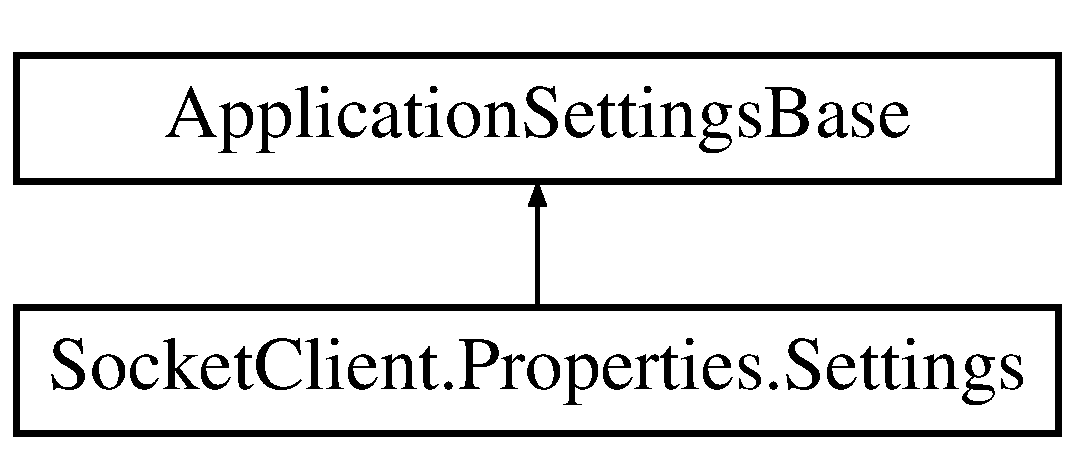
\includegraphics[height=2.000000cm]{class_socket_client_1_1_properties_1_1_settings}
\end{center}
\end{figure}
\subsection*{Properties}
\begin{DoxyCompactItemize}
\item 
static \hyperlink{class_socket_client_1_1_properties_1_1_settings}{Settings} \hyperlink{class_socket_client_1_1_properties_1_1_settings_a052759b480879768820530ea7d850247}{Default}\hspace{0.3cm}{\ttfamily  \mbox{[}get\mbox{]}}
\end{DoxyCompactItemize}
\subsection*{Static Private Attributes}
\begin{DoxyCompactItemize}
\item 
static \hyperlink{class_socket_client_1_1_properties_1_1_settings}{Settings} \hyperlink{class_socket_client_1_1_properties_1_1_settings_a5bc40a9d598e5dfb06cf56795afe980d}{default\+Instance} = ((\hyperlink{class_socket_client_1_1_properties_1_1_settings}{Settings})(global\+::\+System.\+Configuration.\+Application\+Settings\+Base.\+Synchronized(new \hyperlink{class_socket_client_1_1_properties_1_1_settings}{Settings}())))
\end{DoxyCompactItemize}


\subsection{Member Data Documentation}
\mbox{\Hypertarget{class_socket_client_1_1_properties_1_1_settings_a5bc40a9d598e5dfb06cf56795afe980d}\label{class_socket_client_1_1_properties_1_1_settings_a5bc40a9d598e5dfb06cf56795afe980d}} 
\index{Socket\+Client\+::\+Properties\+::\+Settings@{Socket\+Client\+::\+Properties\+::\+Settings}!default\+Instance@{default\+Instance}}
\index{default\+Instance@{default\+Instance}!Socket\+Client\+::\+Properties\+::\+Settings@{Socket\+Client\+::\+Properties\+::\+Settings}}
\subsubsection{\texorpdfstring{default\+Instance}{defaultInstance}}
{\footnotesize\ttfamily \hyperlink{class_socket_client_1_1_properties_1_1_settings}{Settings} Socket\+Client.\+Properties.\+Settings.\+default\+Instance = ((\hyperlink{class_socket_client_1_1_properties_1_1_settings}{Settings})(global\+::\+System.\+Configuration.\+Application\+Settings\+Base.\+Synchronized(new \hyperlink{class_socket_client_1_1_properties_1_1_settings}{Settings}())))\hspace{0.3cm}{\ttfamily [static]}, {\ttfamily [private]}}



\subsection{Property Documentation}
\mbox{\Hypertarget{class_socket_client_1_1_properties_1_1_settings_a052759b480879768820530ea7d850247}\label{class_socket_client_1_1_properties_1_1_settings_a052759b480879768820530ea7d850247}} 
\index{Socket\+Client\+::\+Properties\+::\+Settings@{Socket\+Client\+::\+Properties\+::\+Settings}!Default@{Default}}
\index{Default@{Default}!Socket\+Client\+::\+Properties\+::\+Settings@{Socket\+Client\+::\+Properties\+::\+Settings}}
\subsubsection{\texorpdfstring{Default}{Default}}
{\footnotesize\ttfamily \hyperlink{class_socket_client_1_1_properties_1_1_settings}{Settings} Socket\+Client.\+Properties.\+Settings.\+Default\hspace{0.3cm}{\ttfamily [static]}, {\ttfamily [get]}}



The documentation for this class was generated from the following file\+:\begin{DoxyCompactItemize}
\item 
G\+:/\+Assessment\+Three/\+Assesment\+Three\+Part\+B/\+Socket\+Client/\+Properties/\hyperlink{_socket_client_2_properties_2_settings_8_designer_8cs}{Settings.\+Designer.\+cs}\end{DoxyCompactItemize}

\hypertarget{class_socket_server_1_1_properties_1_1_settings}{}\section{Socket\+Server.\+Properties.\+Settings Class Reference}
\label{class_socket_server_1_1_properties_1_1_settings}\index{Socket\+Server.\+Properties.\+Settings@{Socket\+Server.\+Properties.\+Settings}}
Inheritance diagram for Socket\+Server.\+Properties.\+Settings\+:\begin{figure}[H]
\begin{center}
\leavevmode
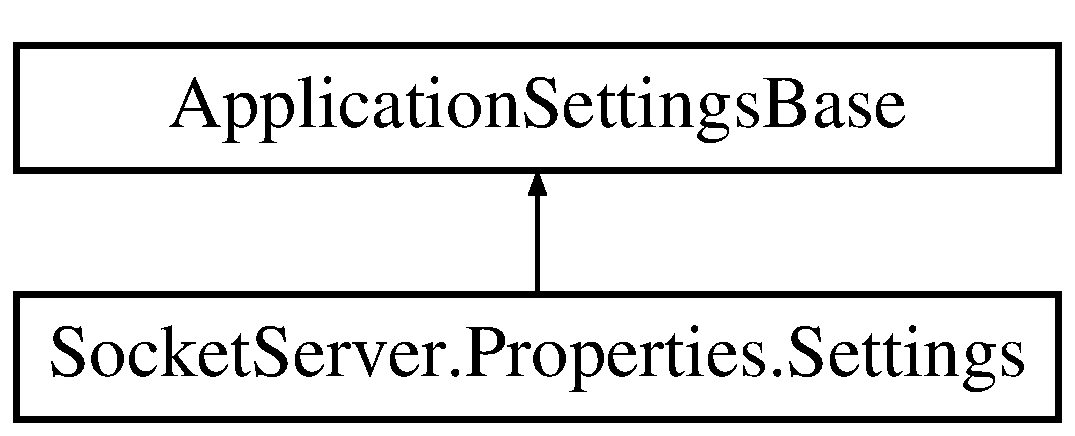
\includegraphics[height=2.000000cm]{class_socket_server_1_1_properties_1_1_settings}
\end{center}
\end{figure}
\subsection*{Properties}
\begin{DoxyCompactItemize}
\item 
static \hyperlink{class_socket_server_1_1_properties_1_1_settings}{Settings} \hyperlink{class_socket_server_1_1_properties_1_1_settings_a7944b37c40f557280d233c0cfa179c2d}{Default}\hspace{0.3cm}{\ttfamily  \mbox{[}get\mbox{]}}
\end{DoxyCompactItemize}
\subsection*{Static Private Attributes}
\begin{DoxyCompactItemize}
\item 
static \hyperlink{class_socket_server_1_1_properties_1_1_settings}{Settings} \hyperlink{class_socket_server_1_1_properties_1_1_settings_a5335d790e0262a7276d3c0879758bd10}{default\+Instance} = ((\hyperlink{class_socket_server_1_1_properties_1_1_settings}{Settings})(global\+::\+System.\+Configuration.\+Application\+Settings\+Base.\+Synchronized(new \hyperlink{class_socket_server_1_1_properties_1_1_settings}{Settings}())))
\end{DoxyCompactItemize}


\subsection{Member Data Documentation}
\mbox{\Hypertarget{class_socket_server_1_1_properties_1_1_settings_a5335d790e0262a7276d3c0879758bd10}\label{class_socket_server_1_1_properties_1_1_settings_a5335d790e0262a7276d3c0879758bd10}} 
\index{Socket\+Server\+::\+Properties\+::\+Settings@{Socket\+Server\+::\+Properties\+::\+Settings}!default\+Instance@{default\+Instance}}
\index{default\+Instance@{default\+Instance}!Socket\+Server\+::\+Properties\+::\+Settings@{Socket\+Server\+::\+Properties\+::\+Settings}}
\subsubsection{\texorpdfstring{default\+Instance}{defaultInstance}}
{\footnotesize\ttfamily \hyperlink{class_socket_server_1_1_properties_1_1_settings}{Settings} Socket\+Server.\+Properties.\+Settings.\+default\+Instance = ((\hyperlink{class_socket_server_1_1_properties_1_1_settings}{Settings})(global\+::\+System.\+Configuration.\+Application\+Settings\+Base.\+Synchronized(new \hyperlink{class_socket_server_1_1_properties_1_1_settings}{Settings}())))\hspace{0.3cm}{\ttfamily [static]}, {\ttfamily [private]}}



\subsection{Property Documentation}
\mbox{\Hypertarget{class_socket_server_1_1_properties_1_1_settings_a7944b37c40f557280d233c0cfa179c2d}\label{class_socket_server_1_1_properties_1_1_settings_a7944b37c40f557280d233c0cfa179c2d}} 
\index{Socket\+Server\+::\+Properties\+::\+Settings@{Socket\+Server\+::\+Properties\+::\+Settings}!Default@{Default}}
\index{Default@{Default}!Socket\+Server\+::\+Properties\+::\+Settings@{Socket\+Server\+::\+Properties\+::\+Settings}}
\subsubsection{\texorpdfstring{Default}{Default}}
{\footnotesize\ttfamily \hyperlink{class_socket_server_1_1_properties_1_1_settings}{Settings} Socket\+Server.\+Properties.\+Settings.\+Default\hspace{0.3cm}{\ttfamily [static]}, {\ttfamily [get]}}



The documentation for this class was generated from the following file\+:\begin{DoxyCompactItemize}
\item 
G\+:/\+Assessment\+Three/\+Assesment\+Three\+Part\+B/\+Socket\+Server/\+Properties/\hyperlink{_socket_server_2_properties_2_settings_8_designer_8cs}{Settings.\+Designer.\+cs}\end{DoxyCompactItemize}

\hypertarget{class_socket_client_1_1_socket_client}{}\section{Socket\+Client.\+Socket\+Client Class Reference}
\label{class_socket_client_1_1_socket_client}\index{Socket\+Client.\+Socket\+Client@{Socket\+Client.\+Socket\+Client}}


Class for client operations.  


Inheritance diagram for Socket\+Client.\+Socket\+Client\+:\begin{figure}[H]
\begin{center}
\leavevmode
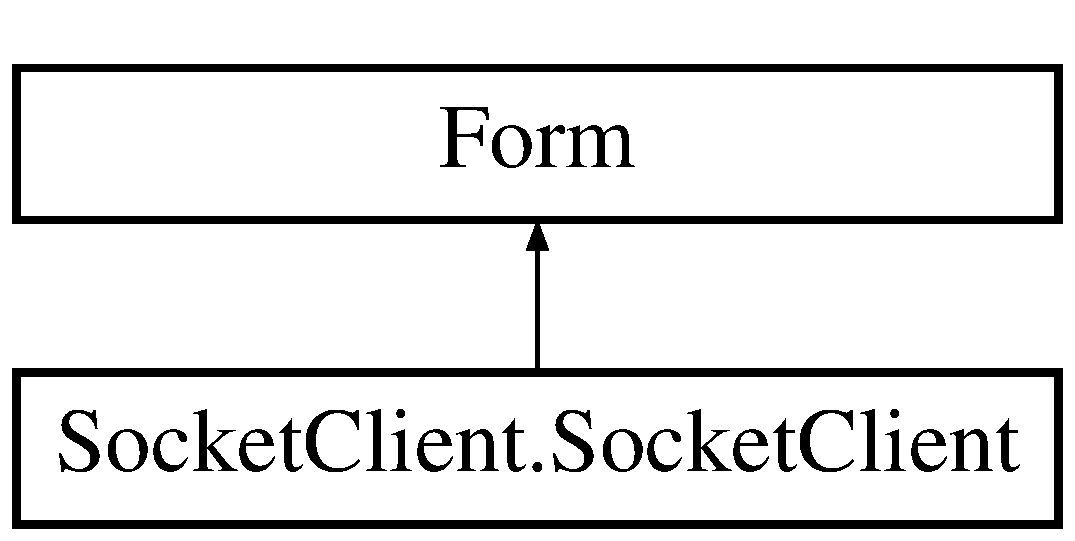
\includegraphics[height=2.000000cm]{class_socket_client_1_1_socket_client}
\end{center}
\end{figure}
\subsection*{Public Member Functions}
\begin{DoxyCompactItemize}
\item 
\hyperlink{class_socket_client_1_1_socket_client_aa6b5f080048da540d30bfe849b1e3260}{Socket\+Client} ()
\end{DoxyCompactItemize}
\subsection*{Protected Member Functions}
\begin{DoxyCompactItemize}
\item 
override void \hyperlink{class_socket_client_1_1_socket_client_ab28be4e020b665a2b8cc879beac14062}{Dispose} (bool disposing)
\begin{DoxyCompactList}\small\item\em Clean up any resources being used. \end{DoxyCompactList}\end{DoxyCompactItemize}
\subsection*{Private Member Functions}
\begin{DoxyCompactItemize}
\item 
void \hyperlink{class_socket_client_1_1_socket_client_a11f3d8e059c5212571ffa31b341db817}{Connect\+Btn\+\_\+\+Click} (object sender, Event\+Args e)
\item 
void \hyperlink{class_socket_client_1_1_socket_client_a9f94765a98f16857de0abb270fbe9679}{Connect\+To\+Callback} (I\+Async\+Result ar)
\item 
void \hyperlink{class_socket_client_1_1_socket_client_ace38e3f7f43d32563ffb8f20cfa9ee19}{Receive\+Callback} (I\+Async\+Result AR)
\item 
void \hyperlink{class_socket_client_1_1_socket_client_aa5bdeccde8564ade04ece861218ba7f3}{Send\+Name} ()
\item 
void \hyperlink{class_socket_client_1_1_socket_client_aa3a0cd25dc845093679adab2eabcf118}{Update\+Control\+States} (bool toggle)
\item 
void \hyperlink{class_socket_client_1_1_socket_client_a9080f6ed9103d3388e3768da4276e237}{Send\+Btn\+\_\+\+Click} (object sender, Event\+Args e)
\item 
void \hyperlink{class_socket_client_1_1_socket_client_a0ffad9543c6accf3fa6a6d957b34feb9}{Send\+Text} (\hyperlink{class_socket_client_1_1_client}{Client} \hyperlink{class_socket_client_1_1_socket_client_a09a6b075aa1a2e8669cf52466e28b988}{client})
\item 
void \hyperlink{class_socket_client_1_1_socket_client_aa1542d2df54e6322e37d87724ff01391}{Exit\+Btn\+\_\+\+Click} (object sender, Event\+Args e)
\item 
void \hyperlink{class_socket_client_1_1_socket_client_a10780b5b665e5f1be462b728be91f253}{Send\+Txt\+\_\+\+Key\+Down} (object sender, Key\+Event\+Args e)
\item 
void \hyperlink{class_socket_client_1_1_socket_client_a0a1cbcdf80431b5be6a9693df1e4933b}{Name\+Txt\+\_\+\+Key\+Down} (object sender, Key\+Event\+Args e)
\item 
void \hyperlink{class_socket_client_1_1_socket_client_ae31dc82e1b1d076129b128b42886be56}{Initialize\+Component} ()
\begin{DoxyCompactList}\small\item\em Required method for Designer support -\/ do not modify the contents of this method with the code editor. \end{DoxyCompactList}\end{DoxyCompactItemize}
\subsection*{Private Attributes}
\begin{DoxyCompactItemize}
\item 
Socket \hyperlink{class_socket_client_1_1_socket_client_a35ccb5352efed508548995ab83a319b7}{m\+Client\+Socket} = new Socket(Address\+Family.\+Inter\+Network, Socket\+Type.\+Stream, Protocol\+Type.\+Tcp)
\item 
\hyperlink{class_socket_client_1_1_client}{Client} \hyperlink{class_socket_client_1_1_socket_client_a09a6b075aa1a2e8669cf52466e28b988}{client}
\begin{DoxyCompactList}\small\item\em declaring an empty instance of \hyperlink{class_socket_client_1_1_client}{Client} \end{DoxyCompactList}\item 
byte \mbox{[}$\,$\mbox{]} \hyperlink{class_socket_client_1_1_socket_client_a0a354f927be0db166f1510a33cc0b13d}{m\+Received\+Data} = new byte\mbox{[}1024\mbox{]}
\begin{DoxyCompactList}\small\item\em byte array to store data received \end{DoxyCompactList}\item 
byte \mbox{[}$\,$\mbox{]} \hyperlink{class_socket_client_1_1_socket_client_aefa3c0bc58365462d700b01447b36d64}{m\+Send\+Data} = new byte\mbox{[}1024\mbox{]}
\begin{DoxyCompactList}\small\item\em byte array to store data send \end{DoxyCompactList}\item 
System.\+Component\+Model.\+I\+Container \hyperlink{class_socket_client_1_1_socket_client_a93c4c9bc725018e23eb8722ff5c5035c}{components} = null
\begin{DoxyCompactList}\small\item\em Required designer variable. \end{DoxyCompactList}\item 
System.\+Windows.\+Forms.\+Text\+Box \hyperlink{class_socket_client_1_1_socket_client_aa6e996e071df29e1290ab24dcc917831}{received\+Txt}
\item 
System.\+Windows.\+Forms.\+Button \hyperlink{class_socket_client_1_1_socket_client_a4189e5451a07ac6a6b7818910e005028}{connect\+Btn}
\item 
System.\+Windows.\+Forms.\+Button \hyperlink{class_socket_client_1_1_socket_client_ae39ef5159c71a2e983b6c19d3548622c}{send\+Btn}
\item 
System.\+Windows.\+Forms.\+Label \hyperlink{class_socket_client_1_1_socket_client_af918eefc5c4d3d78f8238ed2bde0d6b8}{name\+Lbl}
\item 
System.\+Windows.\+Forms.\+Text\+Box \hyperlink{class_socket_client_1_1_socket_client_a88b44242ed0a3716498b1dd4c6f19a39}{name\+Txt}
\item 
System.\+Windows.\+Forms.\+Button \hyperlink{class_socket_client_1_1_socket_client_a6874b1727fc1ddd55e07545e7cd6e28d}{exit\+Btn}
\item 
System.\+Windows.\+Forms.\+Text\+Box \hyperlink{class_socket_client_1_1_socket_client_ae178c12147d21c828bb8a444267289ee}{send\+Txt}
\end{DoxyCompactItemize}


\subsection{Detailed Description}
Class for client operations. 



\subsection{Constructor \& Destructor Documentation}
\mbox{\Hypertarget{class_socket_client_1_1_socket_client_aa6b5f080048da540d30bfe849b1e3260}\label{class_socket_client_1_1_socket_client_aa6b5f080048da540d30bfe849b1e3260}} 
\index{Socket\+Client\+::\+Socket\+Client@{Socket\+Client\+::\+Socket\+Client}!Socket\+Client@{Socket\+Client}}
\index{Socket\+Client@{Socket\+Client}!Socket\+Client\+::\+Socket\+Client@{Socket\+Client\+::\+Socket\+Client}}
\subsubsection{\texorpdfstring{Socket\+Client()}{SocketClient()}}
{\footnotesize\ttfamily Socket\+Client.\+Socket\+Client.\+Socket\+Client (\begin{DoxyParamCaption}{ }\end{DoxyParamCaption})\hspace{0.3cm}{\ttfamily [inline]}}



\subsection{Member Function Documentation}
\mbox{\Hypertarget{class_socket_client_1_1_socket_client_a11f3d8e059c5212571ffa31b341db817}\label{class_socket_client_1_1_socket_client_a11f3d8e059c5212571ffa31b341db817}} 
\index{Socket\+Client\+::\+Socket\+Client@{Socket\+Client\+::\+Socket\+Client}!Connect\+Btn\+\_\+\+Click@{Connect\+Btn\+\_\+\+Click}}
\index{Connect\+Btn\+\_\+\+Click@{Connect\+Btn\+\_\+\+Click}!Socket\+Client\+::\+Socket\+Client@{Socket\+Client\+::\+Socket\+Client}}
\subsubsection{\texorpdfstring{Connect\+Btn\+\_\+\+Click()}{ConnectBtn\_Click()}}
{\footnotesize\ttfamily void Socket\+Client.\+Socket\+Client.\+Connect\+Btn\+\_\+\+Click (\begin{DoxyParamCaption}\item[{object}]{sender,  }\item[{Event\+Args}]{e }\end{DoxyParamCaption})\hspace{0.3cm}{\ttfamily [inline]}, {\ttfamily [private]}}

Function to handle connecting to the server and ensuring a name is entered when the connect button is clicked. \mbox{\Hypertarget{class_socket_client_1_1_socket_client_a9f94765a98f16857de0abb270fbe9679}\label{class_socket_client_1_1_socket_client_a9f94765a98f16857de0abb270fbe9679}} 
\index{Socket\+Client\+::\+Socket\+Client@{Socket\+Client\+::\+Socket\+Client}!Connect\+To\+Callback@{Connect\+To\+Callback}}
\index{Connect\+To\+Callback@{Connect\+To\+Callback}!Socket\+Client\+::\+Socket\+Client@{Socket\+Client\+::\+Socket\+Client}}
\subsubsection{\texorpdfstring{Connect\+To\+Callback()}{ConnectToCallback()}}
{\footnotesize\ttfamily void Socket\+Client.\+Socket\+Client.\+Connect\+To\+Callback (\begin{DoxyParamCaption}\item[{I\+Async\+Result}]{ar }\end{DoxyParamCaption})\hspace{0.3cm}{\ttfamily [inline]}, {\ttfamily [private]}}

Callback function for connecting to a server. \mbox{\Hypertarget{class_socket_client_1_1_socket_client_ab28be4e020b665a2b8cc879beac14062}\label{class_socket_client_1_1_socket_client_ab28be4e020b665a2b8cc879beac14062}} 
\index{Socket\+Client\+::\+Socket\+Client@{Socket\+Client\+::\+Socket\+Client}!Dispose@{Dispose}}
\index{Dispose@{Dispose}!Socket\+Client\+::\+Socket\+Client@{Socket\+Client\+::\+Socket\+Client}}
\subsubsection{\texorpdfstring{Dispose()}{Dispose()}}
{\footnotesize\ttfamily override void Socket\+Client.\+Socket\+Client.\+Dispose (\begin{DoxyParamCaption}\item[{bool}]{disposing }\end{DoxyParamCaption})\hspace{0.3cm}{\ttfamily [inline]}, {\ttfamily [protected]}}



Clean up any resources being used. 


\begin{DoxyParams}{Parameters}
{\em disposing} & true if managed resources should be disposed; otherwise, false.\\
\hline
\end{DoxyParams}
\mbox{\Hypertarget{class_socket_client_1_1_socket_client_aa1542d2df54e6322e37d87724ff01391}\label{class_socket_client_1_1_socket_client_aa1542d2df54e6322e37d87724ff01391}} 
\index{Socket\+Client\+::\+Socket\+Client@{Socket\+Client\+::\+Socket\+Client}!Exit\+Btn\+\_\+\+Click@{Exit\+Btn\+\_\+\+Click}}
\index{Exit\+Btn\+\_\+\+Click@{Exit\+Btn\+\_\+\+Click}!Socket\+Client\+::\+Socket\+Client@{Socket\+Client\+::\+Socket\+Client}}
\subsubsection{\texorpdfstring{Exit\+Btn\+\_\+\+Click()}{ExitBtn\_Click()}}
{\footnotesize\ttfamily void Socket\+Client.\+Socket\+Client.\+Exit\+Btn\+\_\+\+Click (\begin{DoxyParamCaption}\item[{object}]{sender,  }\item[{Event\+Args}]{e }\end{DoxyParamCaption})\hspace{0.3cm}{\ttfamily [inline]}, {\ttfamily [private]}}

Function to handle informing the server of a client disconnecting, closing the socket and quitting the application. \mbox{\Hypertarget{class_socket_client_1_1_socket_client_ae31dc82e1b1d076129b128b42886be56}\label{class_socket_client_1_1_socket_client_ae31dc82e1b1d076129b128b42886be56}} 
\index{Socket\+Client\+::\+Socket\+Client@{Socket\+Client\+::\+Socket\+Client}!Initialize\+Component@{Initialize\+Component}}
\index{Initialize\+Component@{Initialize\+Component}!Socket\+Client\+::\+Socket\+Client@{Socket\+Client\+::\+Socket\+Client}}
\subsubsection{\texorpdfstring{Initialize\+Component()}{InitializeComponent()}}
{\footnotesize\ttfamily void Socket\+Client.\+Socket\+Client.\+Initialize\+Component (\begin{DoxyParamCaption}{ }\end{DoxyParamCaption})\hspace{0.3cm}{\ttfamily [inline]}, {\ttfamily [private]}}



Required method for Designer support -\/ do not modify the contents of this method with the code editor. 

\mbox{\Hypertarget{class_socket_client_1_1_socket_client_a0a1cbcdf80431b5be6a9693df1e4933b}\label{class_socket_client_1_1_socket_client_a0a1cbcdf80431b5be6a9693df1e4933b}} 
\index{Socket\+Client\+::\+Socket\+Client@{Socket\+Client\+::\+Socket\+Client}!Name\+Txt\+\_\+\+Key\+Down@{Name\+Txt\+\_\+\+Key\+Down}}
\index{Name\+Txt\+\_\+\+Key\+Down@{Name\+Txt\+\_\+\+Key\+Down}!Socket\+Client\+::\+Socket\+Client@{Socket\+Client\+::\+Socket\+Client}}
\subsubsection{\texorpdfstring{Name\+Txt\+\_\+\+Key\+Down()}{NameTxt\_KeyDown()}}
{\footnotesize\ttfamily void Socket\+Client.\+Socket\+Client.\+Name\+Txt\+\_\+\+Key\+Down (\begin{DoxyParamCaption}\item[{object}]{sender,  }\item[{Key\+Event\+Args}]{e }\end{DoxyParamCaption})\hspace{0.3cm}{\ttfamily [inline]}, {\ttfamily [private]}}

Function for detecting when the enter key is pressed whilst focused on the name\+Txt textbox and sending the data. \mbox{\Hypertarget{class_socket_client_1_1_socket_client_ace38e3f7f43d32563ffb8f20cfa9ee19}\label{class_socket_client_1_1_socket_client_ace38e3f7f43d32563ffb8f20cfa9ee19}} 
\index{Socket\+Client\+::\+Socket\+Client@{Socket\+Client\+::\+Socket\+Client}!Receive\+Callback@{Receive\+Callback}}
\index{Receive\+Callback@{Receive\+Callback}!Socket\+Client\+::\+Socket\+Client@{Socket\+Client\+::\+Socket\+Client}}
\subsubsection{\texorpdfstring{Receive\+Callback()}{ReceiveCallback()}}
{\footnotesize\ttfamily void Socket\+Client.\+Socket\+Client.\+Receive\+Callback (\begin{DoxyParamCaption}\item[{I\+Async\+Result}]{AR }\end{DoxyParamCaption})\hspace{0.3cm}{\ttfamily [inline]}, {\ttfamily [private]}}

Function for receiving data from the server and displaying the data received in textbox. \mbox{\Hypertarget{class_socket_client_1_1_socket_client_a9080f6ed9103d3388e3768da4276e237}\label{class_socket_client_1_1_socket_client_a9080f6ed9103d3388e3768da4276e237}} 
\index{Socket\+Client\+::\+Socket\+Client@{Socket\+Client\+::\+Socket\+Client}!Send\+Btn\+\_\+\+Click@{Send\+Btn\+\_\+\+Click}}
\index{Send\+Btn\+\_\+\+Click@{Send\+Btn\+\_\+\+Click}!Socket\+Client\+::\+Socket\+Client@{Socket\+Client\+::\+Socket\+Client}}
\subsubsection{\texorpdfstring{Send\+Btn\+\_\+\+Click()}{SendBtn\_Click()}}
{\footnotesize\ttfamily void Socket\+Client.\+Socket\+Client.\+Send\+Btn\+\_\+\+Click (\begin{DoxyParamCaption}\item[{object}]{sender,  }\item[{Event\+Args}]{e }\end{DoxyParamCaption})\hspace{0.3cm}{\ttfamily [inline]}, {\ttfamily [private]}}

Function to handle sending data to the server when the send button is clicked. \mbox{\Hypertarget{class_socket_client_1_1_socket_client_aa5bdeccde8564ade04ece861218ba7f3}\label{class_socket_client_1_1_socket_client_aa5bdeccde8564ade04ece861218ba7f3}} 
\index{Socket\+Client\+::\+Socket\+Client@{Socket\+Client\+::\+Socket\+Client}!Send\+Name@{Send\+Name}}
\index{Send\+Name@{Send\+Name}!Socket\+Client\+::\+Socket\+Client@{Socket\+Client\+::\+Socket\+Client}}
\subsubsection{\texorpdfstring{Send\+Name()}{SendName()}}
{\footnotesize\ttfamily void Socket\+Client.\+Socket\+Client.\+Send\+Name (\begin{DoxyParamCaption}{ }\end{DoxyParamCaption})\hspace{0.3cm}{\ttfamily [inline]}, {\ttfamily [private]}}

Function for sending the clients name upon connection. will only be called once. \mbox{\Hypertarget{class_socket_client_1_1_socket_client_a0ffad9543c6accf3fa6a6d957b34feb9}\label{class_socket_client_1_1_socket_client_a0ffad9543c6accf3fa6a6d957b34feb9}} 
\index{Socket\+Client\+::\+Socket\+Client@{Socket\+Client\+::\+Socket\+Client}!Send\+Text@{Send\+Text}}
\index{Send\+Text@{Send\+Text}!Socket\+Client\+::\+Socket\+Client@{Socket\+Client\+::\+Socket\+Client}}
\subsubsection{\texorpdfstring{Send\+Text()}{SendText()}}
{\footnotesize\ttfamily void Socket\+Client.\+Socket\+Client.\+Send\+Text (\begin{DoxyParamCaption}\item[{\hyperlink{class_socket_client_1_1_client}{Client}}]{client }\end{DoxyParamCaption})\hspace{0.3cm}{\ttfamily [inline]}, {\ttfamily [private]}}

Function for sending client object to the server. \mbox{\Hypertarget{class_socket_client_1_1_socket_client_a10780b5b665e5f1be462b728be91f253}\label{class_socket_client_1_1_socket_client_a10780b5b665e5f1be462b728be91f253}} 
\index{Socket\+Client\+::\+Socket\+Client@{Socket\+Client\+::\+Socket\+Client}!Send\+Txt\+\_\+\+Key\+Down@{Send\+Txt\+\_\+\+Key\+Down}}
\index{Send\+Txt\+\_\+\+Key\+Down@{Send\+Txt\+\_\+\+Key\+Down}!Socket\+Client\+::\+Socket\+Client@{Socket\+Client\+::\+Socket\+Client}}
\subsubsection{\texorpdfstring{Send\+Txt\+\_\+\+Key\+Down()}{SendTxt\_KeyDown()}}
{\footnotesize\ttfamily void Socket\+Client.\+Socket\+Client.\+Send\+Txt\+\_\+\+Key\+Down (\begin{DoxyParamCaption}\item[{object}]{sender,  }\item[{Key\+Event\+Args}]{e }\end{DoxyParamCaption})\hspace{0.3cm}{\ttfamily [inline]}, {\ttfamily [private]}}

Function for detecting when the enter key is pressed whilst focused on the send\+Txt textbox and sending the data. \mbox{\Hypertarget{class_socket_client_1_1_socket_client_aa3a0cd25dc845093679adab2eabcf118}\label{class_socket_client_1_1_socket_client_aa3a0cd25dc845093679adab2eabcf118}} 
\index{Socket\+Client\+::\+Socket\+Client@{Socket\+Client\+::\+Socket\+Client}!Update\+Control\+States@{Update\+Control\+States}}
\index{Update\+Control\+States@{Update\+Control\+States}!Socket\+Client\+::\+Socket\+Client@{Socket\+Client\+::\+Socket\+Client}}
\subsubsection{\texorpdfstring{Update\+Control\+States()}{UpdateControlStates()}}
{\footnotesize\ttfamily void Socket\+Client.\+Socket\+Client.\+Update\+Control\+States (\begin{DoxyParamCaption}\item[{bool}]{toggle }\end{DoxyParamCaption})\hspace{0.3cm}{\ttfamily [inline]}, {\ttfamily [private]}}

Function for toggling controls. 

\subsection{Member Data Documentation}
\mbox{\Hypertarget{class_socket_client_1_1_socket_client_a09a6b075aa1a2e8669cf52466e28b988}\label{class_socket_client_1_1_socket_client_a09a6b075aa1a2e8669cf52466e28b988}} 
\index{Socket\+Client\+::\+Socket\+Client@{Socket\+Client\+::\+Socket\+Client}!client@{client}}
\index{client@{client}!Socket\+Client\+::\+Socket\+Client@{Socket\+Client\+::\+Socket\+Client}}
\subsubsection{\texorpdfstring{client}{client}}
{\footnotesize\ttfamily \hyperlink{class_socket_client_1_1_client}{Client} Socket\+Client.\+Socket\+Client.\+client\hspace{0.3cm}{\ttfamily [private]}}



declaring an empty instance of \hyperlink{class_socket_client_1_1_client}{Client} 

\mbox{\Hypertarget{class_socket_client_1_1_socket_client_a93c4c9bc725018e23eb8722ff5c5035c}\label{class_socket_client_1_1_socket_client_a93c4c9bc725018e23eb8722ff5c5035c}} 
\index{Socket\+Client\+::\+Socket\+Client@{Socket\+Client\+::\+Socket\+Client}!components@{components}}
\index{components@{components}!Socket\+Client\+::\+Socket\+Client@{Socket\+Client\+::\+Socket\+Client}}
\subsubsection{\texorpdfstring{components}{components}}
{\footnotesize\ttfamily System.\+Component\+Model.\+I\+Container Socket\+Client.\+Socket\+Client.\+components = null\hspace{0.3cm}{\ttfamily [private]}}



Required designer variable. 

\mbox{\Hypertarget{class_socket_client_1_1_socket_client_a4189e5451a07ac6a6b7818910e005028}\label{class_socket_client_1_1_socket_client_a4189e5451a07ac6a6b7818910e005028}} 
\index{Socket\+Client\+::\+Socket\+Client@{Socket\+Client\+::\+Socket\+Client}!connect\+Btn@{connect\+Btn}}
\index{connect\+Btn@{connect\+Btn}!Socket\+Client\+::\+Socket\+Client@{Socket\+Client\+::\+Socket\+Client}}
\subsubsection{\texorpdfstring{connect\+Btn}{connectBtn}}
{\footnotesize\ttfamily System.\+Windows.\+Forms.\+Button Socket\+Client.\+Socket\+Client.\+connect\+Btn\hspace{0.3cm}{\ttfamily [private]}}

\mbox{\Hypertarget{class_socket_client_1_1_socket_client_a6874b1727fc1ddd55e07545e7cd6e28d}\label{class_socket_client_1_1_socket_client_a6874b1727fc1ddd55e07545e7cd6e28d}} 
\index{Socket\+Client\+::\+Socket\+Client@{Socket\+Client\+::\+Socket\+Client}!exit\+Btn@{exit\+Btn}}
\index{exit\+Btn@{exit\+Btn}!Socket\+Client\+::\+Socket\+Client@{Socket\+Client\+::\+Socket\+Client}}
\subsubsection{\texorpdfstring{exit\+Btn}{exitBtn}}
{\footnotesize\ttfamily System.\+Windows.\+Forms.\+Button Socket\+Client.\+Socket\+Client.\+exit\+Btn\hspace{0.3cm}{\ttfamily [private]}}

\mbox{\Hypertarget{class_socket_client_1_1_socket_client_a35ccb5352efed508548995ab83a319b7}\label{class_socket_client_1_1_socket_client_a35ccb5352efed508548995ab83a319b7}} 
\index{Socket\+Client\+::\+Socket\+Client@{Socket\+Client\+::\+Socket\+Client}!m\+Client\+Socket@{m\+Client\+Socket}}
\index{m\+Client\+Socket@{m\+Client\+Socket}!Socket\+Client\+::\+Socket\+Client@{Socket\+Client\+::\+Socket\+Client}}
\subsubsection{\texorpdfstring{m\+Client\+Socket}{mClientSocket}}
{\footnotesize\ttfamily Socket Socket\+Client.\+Socket\+Client.\+m\+Client\+Socket = new Socket(Address\+Family.\+Inter\+Network, Socket\+Type.\+Stream, Protocol\+Type.\+Tcp)\hspace{0.3cm}{\ttfamily [private]}}

\mbox{\Hypertarget{class_socket_client_1_1_socket_client_a0a354f927be0db166f1510a33cc0b13d}\label{class_socket_client_1_1_socket_client_a0a354f927be0db166f1510a33cc0b13d}} 
\index{Socket\+Client\+::\+Socket\+Client@{Socket\+Client\+::\+Socket\+Client}!m\+Received\+Data@{m\+Received\+Data}}
\index{m\+Received\+Data@{m\+Received\+Data}!Socket\+Client\+::\+Socket\+Client@{Socket\+Client\+::\+Socket\+Client}}
\subsubsection{\texorpdfstring{m\+Received\+Data}{mReceivedData}}
{\footnotesize\ttfamily byte \mbox{[}$\,$\mbox{]} Socket\+Client.\+Socket\+Client.\+m\+Received\+Data = new byte\mbox{[}1024\mbox{]}\hspace{0.3cm}{\ttfamily [private]}}



byte array to store data received 

\mbox{\Hypertarget{class_socket_client_1_1_socket_client_aefa3c0bc58365462d700b01447b36d64}\label{class_socket_client_1_1_socket_client_aefa3c0bc58365462d700b01447b36d64}} 
\index{Socket\+Client\+::\+Socket\+Client@{Socket\+Client\+::\+Socket\+Client}!m\+Send\+Data@{m\+Send\+Data}}
\index{m\+Send\+Data@{m\+Send\+Data}!Socket\+Client\+::\+Socket\+Client@{Socket\+Client\+::\+Socket\+Client}}
\subsubsection{\texorpdfstring{m\+Send\+Data}{mSendData}}
{\footnotesize\ttfamily byte \mbox{[}$\,$\mbox{]} Socket\+Client.\+Socket\+Client.\+m\+Send\+Data = new byte\mbox{[}1024\mbox{]}\hspace{0.3cm}{\ttfamily [private]}}



byte array to store data send 

\mbox{\Hypertarget{class_socket_client_1_1_socket_client_af918eefc5c4d3d78f8238ed2bde0d6b8}\label{class_socket_client_1_1_socket_client_af918eefc5c4d3d78f8238ed2bde0d6b8}} 
\index{Socket\+Client\+::\+Socket\+Client@{Socket\+Client\+::\+Socket\+Client}!name\+Lbl@{name\+Lbl}}
\index{name\+Lbl@{name\+Lbl}!Socket\+Client\+::\+Socket\+Client@{Socket\+Client\+::\+Socket\+Client}}
\subsubsection{\texorpdfstring{name\+Lbl}{nameLbl}}
{\footnotesize\ttfamily System.\+Windows.\+Forms.\+Label Socket\+Client.\+Socket\+Client.\+name\+Lbl\hspace{0.3cm}{\ttfamily [private]}}

\mbox{\Hypertarget{class_socket_client_1_1_socket_client_a88b44242ed0a3716498b1dd4c6f19a39}\label{class_socket_client_1_1_socket_client_a88b44242ed0a3716498b1dd4c6f19a39}} 
\index{Socket\+Client\+::\+Socket\+Client@{Socket\+Client\+::\+Socket\+Client}!name\+Txt@{name\+Txt}}
\index{name\+Txt@{name\+Txt}!Socket\+Client\+::\+Socket\+Client@{Socket\+Client\+::\+Socket\+Client}}
\subsubsection{\texorpdfstring{name\+Txt}{nameTxt}}
{\footnotesize\ttfamily System.\+Windows.\+Forms.\+Text\+Box Socket\+Client.\+Socket\+Client.\+name\+Txt\hspace{0.3cm}{\ttfamily [private]}}

\mbox{\Hypertarget{class_socket_client_1_1_socket_client_aa6e996e071df29e1290ab24dcc917831}\label{class_socket_client_1_1_socket_client_aa6e996e071df29e1290ab24dcc917831}} 
\index{Socket\+Client\+::\+Socket\+Client@{Socket\+Client\+::\+Socket\+Client}!received\+Txt@{received\+Txt}}
\index{received\+Txt@{received\+Txt}!Socket\+Client\+::\+Socket\+Client@{Socket\+Client\+::\+Socket\+Client}}
\subsubsection{\texorpdfstring{received\+Txt}{receivedTxt}}
{\footnotesize\ttfamily System.\+Windows.\+Forms.\+Text\+Box Socket\+Client.\+Socket\+Client.\+received\+Txt\hspace{0.3cm}{\ttfamily [private]}}

\mbox{\Hypertarget{class_socket_client_1_1_socket_client_ae39ef5159c71a2e983b6c19d3548622c}\label{class_socket_client_1_1_socket_client_ae39ef5159c71a2e983b6c19d3548622c}} 
\index{Socket\+Client\+::\+Socket\+Client@{Socket\+Client\+::\+Socket\+Client}!send\+Btn@{send\+Btn}}
\index{send\+Btn@{send\+Btn}!Socket\+Client\+::\+Socket\+Client@{Socket\+Client\+::\+Socket\+Client}}
\subsubsection{\texorpdfstring{send\+Btn}{sendBtn}}
{\footnotesize\ttfamily System.\+Windows.\+Forms.\+Button Socket\+Client.\+Socket\+Client.\+send\+Btn\hspace{0.3cm}{\ttfamily [private]}}

\mbox{\Hypertarget{class_socket_client_1_1_socket_client_ae178c12147d21c828bb8a444267289ee}\label{class_socket_client_1_1_socket_client_ae178c12147d21c828bb8a444267289ee}} 
\index{Socket\+Client\+::\+Socket\+Client@{Socket\+Client\+::\+Socket\+Client}!send\+Txt@{send\+Txt}}
\index{send\+Txt@{send\+Txt}!Socket\+Client\+::\+Socket\+Client@{Socket\+Client\+::\+Socket\+Client}}
\subsubsection{\texorpdfstring{send\+Txt}{sendTxt}}
{\footnotesize\ttfamily System.\+Windows.\+Forms.\+Text\+Box Socket\+Client.\+Socket\+Client.\+send\+Txt\hspace{0.3cm}{\ttfamily [private]}}



The documentation for this class was generated from the following files\+:\begin{DoxyCompactItemize}
\item 
G\+:/\+Assessment\+Three/\+Assessment\+Three\+Part\+B/\+Socket\+Client/\hyperlink{_socket_client_8cs}{Socket\+Client.\+cs}\item 
G\+:/\+Assessment\+Three/\+Assessment\+Three\+Part\+B/\+Socket\+Client/\hyperlink{_socket_client_8_designer_8cs}{Socket\+Client.\+Designer.\+cs}\end{DoxyCompactItemize}

\hypertarget{class_socket_server_1_1_socket_server}{}\section{Socket\+Server.\+Socket\+Server Class Reference}
\label{class_socket_server_1_1_socket_server}\index{Socket\+Server.\+Socket\+Server@{Socket\+Server.\+Socket\+Server}}


Class for server operations  


Inheritance diagram for Socket\+Server.\+Socket\+Server\+:\begin{figure}[H]
\begin{center}
\leavevmode
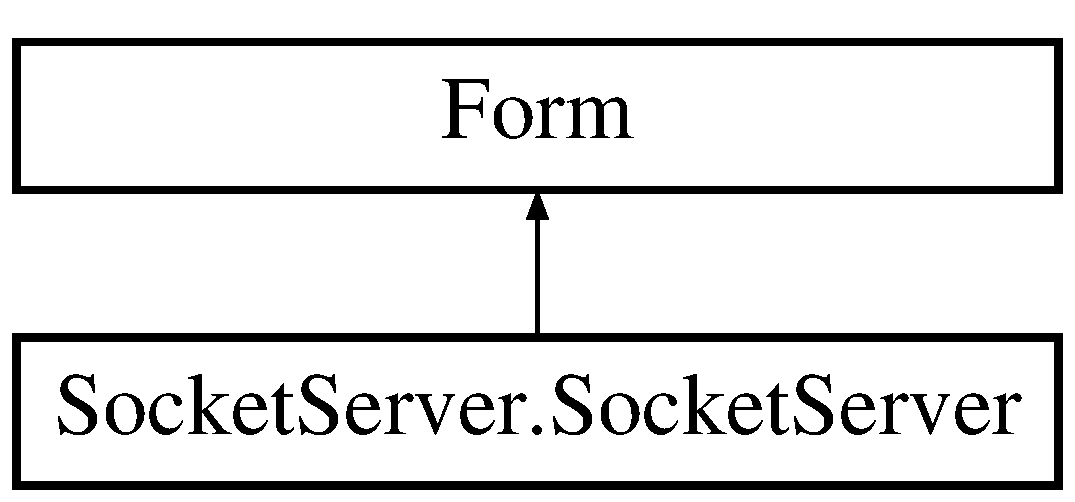
\includegraphics[height=2.000000cm]{class_socket_server_1_1_socket_server}
\end{center}
\end{figure}
\subsection*{Public Member Functions}
\begin{DoxyCompactItemize}
\item 
\hyperlink{class_socket_server_1_1_socket_server_a3f04ad72de3cc8570741afd76a169e4d}{Socket\+Server} ()
\end{DoxyCompactItemize}
\subsection*{Protected Member Functions}
\begin{DoxyCompactItemize}
\item 
override void \hyperlink{class_socket_server_1_1_socket_server_a577f703fecf496140d420e0049159905}{Dispose} (bool disposing)
\begin{DoxyCompactList}\small\item\em Clean up any resources being used. \end{DoxyCompactList}\end{DoxyCompactItemize}
\subsection*{Private Member Functions}
\begin{DoxyCompactItemize}
\item 
void \hyperlink{class_socket_server_1_1_socket_server_a7f3eb3d21566ae27786debe88c434cab}{Setup\+Server} ()
\item 
void \hyperlink{class_socket_server_1_1_socket_server_addf45af964dc6d234b98c719eb7d7a6e}{Accept\+Callback} (I\+Async\+Result ar)
\item 
void \hyperlink{class_socket_server_1_1_socket_server_a03c9fa5afc778edc51344fe0b05730c8}{Recieve\+Name\+Callback} (I\+Async\+Result ar)
\item 
void \hyperlink{class_socket_server_1_1_socket_server_abc93c9ce76d2cc65a209b5144f4bcc74}{Recieve\+Callback} (I\+Async\+Result ar)
\item 
int \hyperlink{class_socket_server_1_1_socket_server_a927514acb2fcf8804b360ad07b677a53}{Update\+Index} (Socket socket)
\item 
void \hyperlink{class_socket_server_1_1_socket_server_a19cb5f0314ec00e0837a893f079bf78d}{Initialize\+Component} ()
\begin{DoxyCompactList}\small\item\em Required method for Designer support -\/ do not modify the contents of this method with the code editor. \end{DoxyCompactList}\end{DoxyCompactItemize}
\subsection*{Private Attributes}
\begin{DoxyCompactItemize}
\item 
Socket \hyperlink{class_socket_server_1_1_socket_server_a3f7c25cca8eb9e7e98dc5172368e8f62}{m\+Server\+Socket} = new Socket(Address\+Family.\+Inter\+Network, Socket\+Type.\+Stream, Protocol\+Type.\+Tcp)
\item 
\hyperlink{class_socket_server_1_1_client}{Client} \hyperlink{class_socket_server_1_1_socket_server_a2c56e560fbab349d4ed56524f1f52f9c}{client}
\begin{DoxyCompactList}\small\item\em declaring an empty instance of \hyperlink{class_socket_server_1_1_client}{Client} \end{DoxyCompactList}\item 
byte \mbox{[}$\,$\mbox{]} \hyperlink{class_socket_server_1_1_socket_server_a989b1e8fe5855a949087d7406db74988}{m\+Received\+Data} = new byte\mbox{[}1024\mbox{]}
\begin{DoxyCompactList}\small\item\em byte array to store data received \end{DoxyCompactList}\item 
byte \mbox{[}$\,$\mbox{]} \hyperlink{class_socket_server_1_1_socket_server_abd27451304549844ef2d93051764fc1a}{m\+Send\+Data} = new byte\mbox{[}1024\mbox{]}
\begin{DoxyCompactList}\small\item\em byte array to store data send \end{DoxyCompactList}\item 
List$<$ \hyperlink{class_socket_server_1_1_client}{Client} $>$ \hyperlink{class_socket_server_1_1_socket_server_ac9461bfbf488d01d0563f1ceb538f4c7}{m\+Clients} = new List$<$\hyperlink{class_socket_server_1_1_client}{Client}$>$()
\begin{DoxyCompactList}\small\item\em list to store clients \end{DoxyCompactList}\item 
List$<$ Socket $>$ \hyperlink{class_socket_server_1_1_socket_server_a7333cc07bf0a885bb0f62f7ecc665742}{m\+Client\+Sockets} = new List$<$Socket$>$()
\begin{DoxyCompactList}\small\item\em list to store client sockets \end{DoxyCompactList}\item 
System.\+Component\+Model.\+I\+Container \hyperlink{class_socket_server_1_1_socket_server_a323fc298b887e4f0f1d764662203703b}{components} = null
\begin{DoxyCompactList}\small\item\em Required designer variable. \end{DoxyCompactList}\item 
System.\+Windows.\+Forms.\+Text\+Box \hyperlink{class_socket_server_1_1_socket_server_aea45323bf62d2f24f8992a0380fd1044}{received\+Txt}
\end{DoxyCompactItemize}


\subsection{Detailed Description}
Class for server operations 



\subsection{Constructor \& Destructor Documentation}
\mbox{\Hypertarget{class_socket_server_1_1_socket_server_a3f04ad72de3cc8570741afd76a169e4d}\label{class_socket_server_1_1_socket_server_a3f04ad72de3cc8570741afd76a169e4d}} 
\index{Socket\+Server\+::\+Socket\+Server@{Socket\+Server\+::\+Socket\+Server}!Socket\+Server@{Socket\+Server}}
\index{Socket\+Server@{Socket\+Server}!Socket\+Server\+::\+Socket\+Server@{Socket\+Server\+::\+Socket\+Server}}
\subsubsection{\texorpdfstring{Socket\+Server()}{SocketServer()}}
{\footnotesize\ttfamily Socket\+Server.\+Socket\+Server.\+Socket\+Server (\begin{DoxyParamCaption}{ }\end{DoxyParamCaption})\hspace{0.3cm}{\ttfamily [inline]}}



\subsection{Member Function Documentation}
\mbox{\Hypertarget{class_socket_server_1_1_socket_server_addf45af964dc6d234b98c719eb7d7a6e}\label{class_socket_server_1_1_socket_server_addf45af964dc6d234b98c719eb7d7a6e}} 
\index{Socket\+Server\+::\+Socket\+Server@{Socket\+Server\+::\+Socket\+Server}!Accept\+Callback@{Accept\+Callback}}
\index{Accept\+Callback@{Accept\+Callback}!Socket\+Server\+::\+Socket\+Server@{Socket\+Server\+::\+Socket\+Server}}
\subsubsection{\texorpdfstring{Accept\+Callback()}{AcceptCallback()}}
{\footnotesize\ttfamily void Socket\+Server.\+Socket\+Server.\+Accept\+Callback (\begin{DoxyParamCaption}\item[{I\+Async\+Result}]{ar }\end{DoxyParamCaption})\hspace{0.3cm}{\ttfamily [inline]}, {\ttfamily [private]}}

when the server receives a connect to callback from a client it accepts it and adds that socket to the list of sockets \mbox{\Hypertarget{class_socket_server_1_1_socket_server_a577f703fecf496140d420e0049159905}\label{class_socket_server_1_1_socket_server_a577f703fecf496140d420e0049159905}} 
\index{Socket\+Server\+::\+Socket\+Server@{Socket\+Server\+::\+Socket\+Server}!Dispose@{Dispose}}
\index{Dispose@{Dispose}!Socket\+Server\+::\+Socket\+Server@{Socket\+Server\+::\+Socket\+Server}}
\subsubsection{\texorpdfstring{Dispose()}{Dispose()}}
{\footnotesize\ttfamily override void Socket\+Server.\+Socket\+Server.\+Dispose (\begin{DoxyParamCaption}\item[{bool}]{disposing }\end{DoxyParamCaption})\hspace{0.3cm}{\ttfamily [inline]}, {\ttfamily [protected]}}



Clean up any resources being used. 


\begin{DoxyParams}{Parameters}
{\em disposing} & true if managed resources should be disposed; otherwise, false.\\
\hline
\end{DoxyParams}
\mbox{\Hypertarget{class_socket_server_1_1_socket_server_a19cb5f0314ec00e0837a893f079bf78d}\label{class_socket_server_1_1_socket_server_a19cb5f0314ec00e0837a893f079bf78d}} 
\index{Socket\+Server\+::\+Socket\+Server@{Socket\+Server\+::\+Socket\+Server}!Initialize\+Component@{Initialize\+Component}}
\index{Initialize\+Component@{Initialize\+Component}!Socket\+Server\+::\+Socket\+Server@{Socket\+Server\+::\+Socket\+Server}}
\subsubsection{\texorpdfstring{Initialize\+Component()}{InitializeComponent()}}
{\footnotesize\ttfamily void Socket\+Server.\+Socket\+Server.\+Initialize\+Component (\begin{DoxyParamCaption}{ }\end{DoxyParamCaption})\hspace{0.3cm}{\ttfamily [inline]}, {\ttfamily [private]}}



Required method for Designer support -\/ do not modify the contents of this method with the code editor. 

\mbox{\Hypertarget{class_socket_server_1_1_socket_server_abc93c9ce76d2cc65a209b5144f4bcc74}\label{class_socket_server_1_1_socket_server_abc93c9ce76d2cc65a209b5144f4bcc74}} 
\index{Socket\+Server\+::\+Socket\+Server@{Socket\+Server\+::\+Socket\+Server}!Recieve\+Callback@{Recieve\+Callback}}
\index{Recieve\+Callback@{Recieve\+Callback}!Socket\+Server\+::\+Socket\+Server@{Socket\+Server\+::\+Socket\+Server}}
\subsubsection{\texorpdfstring{Recieve\+Callback()}{RecieveCallback()}}
{\footnotesize\ttfamily void Socket\+Server.\+Socket\+Server.\+Recieve\+Callback (\begin{DoxyParamCaption}\item[{I\+Async\+Result}]{ar }\end{DoxyParamCaption})\hspace{0.3cm}{\ttfamily [inline]}, {\ttfamily [private]}}

method for handling all text sent from a client \mbox{\Hypertarget{class_socket_server_1_1_socket_server_a03c9fa5afc778edc51344fe0b05730c8}\label{class_socket_server_1_1_socket_server_a03c9fa5afc778edc51344fe0b05730c8}} 
\index{Socket\+Server\+::\+Socket\+Server@{Socket\+Server\+::\+Socket\+Server}!Recieve\+Name\+Callback@{Recieve\+Name\+Callback}}
\index{Recieve\+Name\+Callback@{Recieve\+Name\+Callback}!Socket\+Server\+::\+Socket\+Server@{Socket\+Server\+::\+Socket\+Server}}
\subsubsection{\texorpdfstring{Recieve\+Name\+Callback()}{RecieveNameCallback()}}
{\footnotesize\ttfamily void Socket\+Server.\+Socket\+Server.\+Recieve\+Name\+Callback (\begin{DoxyParamCaption}\item[{I\+Async\+Result}]{ar }\end{DoxyParamCaption})\hspace{0.3cm}{\ttfamily [inline]}, {\ttfamily [private]}}

this method handles receiving name data from the client and printing that name, only called once upon a client connecting \mbox{\Hypertarget{class_socket_server_1_1_socket_server_a7f3eb3d21566ae27786debe88c434cab}\label{class_socket_server_1_1_socket_server_a7f3eb3d21566ae27786debe88c434cab}} 
\index{Socket\+Server\+::\+Socket\+Server@{Socket\+Server\+::\+Socket\+Server}!Setup\+Server@{Setup\+Server}}
\index{Setup\+Server@{Setup\+Server}!Socket\+Server\+::\+Socket\+Server@{Socket\+Server\+::\+Socket\+Server}}
\subsubsection{\texorpdfstring{Setup\+Server()}{SetupServer()}}
{\footnotesize\ttfamily void Socket\+Server.\+Socket\+Server.\+Setup\+Server (\begin{DoxyParamCaption}{ }\end{DoxyParamCaption})\hspace{0.3cm}{\ttfamily [inline]}, {\ttfamily [private]}}

function to set up server which will allow the connection of 2 clients on the port 955 and will take any local ip address \mbox{\Hypertarget{class_socket_server_1_1_socket_server_a927514acb2fcf8804b360ad07b677a53}\label{class_socket_server_1_1_socket_server_a927514acb2fcf8804b360ad07b677a53}} 
\index{Socket\+Server\+::\+Socket\+Server@{Socket\+Server\+::\+Socket\+Server}!Update\+Index@{Update\+Index}}
\index{Update\+Index@{Update\+Index}!Socket\+Server\+::\+Socket\+Server@{Socket\+Server\+::\+Socket\+Server}}
\subsubsection{\texorpdfstring{Update\+Index()}{UpdateIndex()}}
{\footnotesize\ttfamily int Socket\+Server.\+Socket\+Server.\+Update\+Index (\begin{DoxyParamCaption}\item[{Socket}]{socket }\end{DoxyParamCaption})\hspace{0.3cm}{\ttfamily [inline]}, {\ttfamily [private]}}

method to find the index of a current socket 
\begin{DoxyParams}{Parameters}
{\em socket} & the current socket \\
\hline
\end{DoxyParams}


\subsection{Member Data Documentation}
\mbox{\Hypertarget{class_socket_server_1_1_socket_server_a2c56e560fbab349d4ed56524f1f52f9c}\label{class_socket_server_1_1_socket_server_a2c56e560fbab349d4ed56524f1f52f9c}} 
\index{Socket\+Server\+::\+Socket\+Server@{Socket\+Server\+::\+Socket\+Server}!client@{client}}
\index{client@{client}!Socket\+Server\+::\+Socket\+Server@{Socket\+Server\+::\+Socket\+Server}}
\subsubsection{\texorpdfstring{client}{client}}
{\footnotesize\ttfamily \hyperlink{class_socket_server_1_1_client}{Client} Socket\+Server.\+Socket\+Server.\+client\hspace{0.3cm}{\ttfamily [private]}}



declaring an empty instance of \hyperlink{class_socket_server_1_1_client}{Client} 

\mbox{\Hypertarget{class_socket_server_1_1_socket_server_a323fc298b887e4f0f1d764662203703b}\label{class_socket_server_1_1_socket_server_a323fc298b887e4f0f1d764662203703b}} 
\index{Socket\+Server\+::\+Socket\+Server@{Socket\+Server\+::\+Socket\+Server}!components@{components}}
\index{components@{components}!Socket\+Server\+::\+Socket\+Server@{Socket\+Server\+::\+Socket\+Server}}
\subsubsection{\texorpdfstring{components}{components}}
{\footnotesize\ttfamily System.\+Component\+Model.\+I\+Container Socket\+Server.\+Socket\+Server.\+components = null\hspace{0.3cm}{\ttfamily [private]}}



Required designer variable. 

\mbox{\Hypertarget{class_socket_server_1_1_socket_server_ac9461bfbf488d01d0563f1ceb538f4c7}\label{class_socket_server_1_1_socket_server_ac9461bfbf488d01d0563f1ceb538f4c7}} 
\index{Socket\+Server\+::\+Socket\+Server@{Socket\+Server\+::\+Socket\+Server}!m\+Clients@{m\+Clients}}
\index{m\+Clients@{m\+Clients}!Socket\+Server\+::\+Socket\+Server@{Socket\+Server\+::\+Socket\+Server}}
\subsubsection{\texorpdfstring{m\+Clients}{mClients}}
{\footnotesize\ttfamily List$<$\hyperlink{class_socket_server_1_1_client}{Client}$>$ Socket\+Server.\+Socket\+Server.\+m\+Clients = new List$<$\hyperlink{class_socket_server_1_1_client}{Client}$>$()\hspace{0.3cm}{\ttfamily [private]}}



list to store clients 

\mbox{\Hypertarget{class_socket_server_1_1_socket_server_a7333cc07bf0a885bb0f62f7ecc665742}\label{class_socket_server_1_1_socket_server_a7333cc07bf0a885bb0f62f7ecc665742}} 
\index{Socket\+Server\+::\+Socket\+Server@{Socket\+Server\+::\+Socket\+Server}!m\+Client\+Sockets@{m\+Client\+Sockets}}
\index{m\+Client\+Sockets@{m\+Client\+Sockets}!Socket\+Server\+::\+Socket\+Server@{Socket\+Server\+::\+Socket\+Server}}
\subsubsection{\texorpdfstring{m\+Client\+Sockets}{mClientSockets}}
{\footnotesize\ttfamily List$<$Socket$>$ Socket\+Server.\+Socket\+Server.\+m\+Client\+Sockets = new List$<$Socket$>$()\hspace{0.3cm}{\ttfamily [private]}}



list to store client sockets 

\mbox{\Hypertarget{class_socket_server_1_1_socket_server_a989b1e8fe5855a949087d7406db74988}\label{class_socket_server_1_1_socket_server_a989b1e8fe5855a949087d7406db74988}} 
\index{Socket\+Server\+::\+Socket\+Server@{Socket\+Server\+::\+Socket\+Server}!m\+Received\+Data@{m\+Received\+Data}}
\index{m\+Received\+Data@{m\+Received\+Data}!Socket\+Server\+::\+Socket\+Server@{Socket\+Server\+::\+Socket\+Server}}
\subsubsection{\texorpdfstring{m\+Received\+Data}{mReceivedData}}
{\footnotesize\ttfamily byte \mbox{[}$\,$\mbox{]} Socket\+Server.\+Socket\+Server.\+m\+Received\+Data = new byte\mbox{[}1024\mbox{]}\hspace{0.3cm}{\ttfamily [private]}}



byte array to store data received 

\mbox{\Hypertarget{class_socket_server_1_1_socket_server_abd27451304549844ef2d93051764fc1a}\label{class_socket_server_1_1_socket_server_abd27451304549844ef2d93051764fc1a}} 
\index{Socket\+Server\+::\+Socket\+Server@{Socket\+Server\+::\+Socket\+Server}!m\+Send\+Data@{m\+Send\+Data}}
\index{m\+Send\+Data@{m\+Send\+Data}!Socket\+Server\+::\+Socket\+Server@{Socket\+Server\+::\+Socket\+Server}}
\subsubsection{\texorpdfstring{m\+Send\+Data}{mSendData}}
{\footnotesize\ttfamily byte \mbox{[}$\,$\mbox{]} Socket\+Server.\+Socket\+Server.\+m\+Send\+Data = new byte\mbox{[}1024\mbox{]}\hspace{0.3cm}{\ttfamily [private]}}



byte array to store data send 

\mbox{\Hypertarget{class_socket_server_1_1_socket_server_a3f7c25cca8eb9e7e98dc5172368e8f62}\label{class_socket_server_1_1_socket_server_a3f7c25cca8eb9e7e98dc5172368e8f62}} 
\index{Socket\+Server\+::\+Socket\+Server@{Socket\+Server\+::\+Socket\+Server}!m\+Server\+Socket@{m\+Server\+Socket}}
\index{m\+Server\+Socket@{m\+Server\+Socket}!Socket\+Server\+::\+Socket\+Server@{Socket\+Server\+::\+Socket\+Server}}
\subsubsection{\texorpdfstring{m\+Server\+Socket}{mServerSocket}}
{\footnotesize\ttfamily Socket Socket\+Server.\+Socket\+Server.\+m\+Server\+Socket = new Socket(Address\+Family.\+Inter\+Network, Socket\+Type.\+Stream, Protocol\+Type.\+Tcp)\hspace{0.3cm}{\ttfamily [private]}}

\mbox{\Hypertarget{class_socket_server_1_1_socket_server_aea45323bf62d2f24f8992a0380fd1044}\label{class_socket_server_1_1_socket_server_aea45323bf62d2f24f8992a0380fd1044}} 
\index{Socket\+Server\+::\+Socket\+Server@{Socket\+Server\+::\+Socket\+Server}!received\+Txt@{received\+Txt}}
\index{received\+Txt@{received\+Txt}!Socket\+Server\+::\+Socket\+Server@{Socket\+Server\+::\+Socket\+Server}}
\subsubsection{\texorpdfstring{received\+Txt}{receivedTxt}}
{\footnotesize\ttfamily System.\+Windows.\+Forms.\+Text\+Box Socket\+Server.\+Socket\+Server.\+received\+Txt\hspace{0.3cm}{\ttfamily [private]}}



The documentation for this class was generated from the following files\+:\begin{DoxyCompactItemize}
\item 
G\+:/\+Assessment\+Three/\+Assesment\+Three\+Part\+B/\+Socket\+Server/\hyperlink{_socket_server_8cs}{Socket\+Server.\+cs}\item 
G\+:/\+Assessment\+Three/\+Assesment\+Three\+Part\+B/\+Socket\+Server/\hyperlink{_socket_server_8_designer_8cs}{Socket\+Server.\+Designer.\+cs}\end{DoxyCompactItemize}

\chapter{File Documentation}
\hypertarget{_app_functions_8cs}{}\section{G\+:/\+Assessment\+Three/\+Assesment\+Three\+Part\+B/\+Socket\+Client/\+App\+Functions.cs File Reference}
\label{_app_functions_8cs}\index{G\+:/\+Assessment\+Three/\+Assesment\+Three\+Part\+B/\+Socket\+Client/\+App\+Functions.\+cs@{G\+:/\+Assessment\+Three/\+Assesment\+Three\+Part\+B/\+Socket\+Client/\+App\+Functions.\+cs}}
\subsection*{Classes}
\begin{DoxyCompactItemize}
\item 
class \hyperlink{class_socket_client_1_1_app_functions}{Socket\+Client.\+App\+Functions}
\begin{DoxyCompactList}\small\item\em static class for methods that can be used in both \hyperlink{class_socket_client_1_1_socket_client}{Socket\+Client} and \hyperlink{namespace_socket_server}{Socket\+Server} classes \end{DoxyCompactList}\end{DoxyCompactItemize}
\subsection*{Namespaces}
\begin{DoxyCompactItemize}
\item 
namespace \hyperlink{namespace_socket_client}{Socket\+Client}
\end{DoxyCompactItemize}

\hypertarget{_socket_client_2_client_8cs}{}\section{G\+:/\+Assessment\+Three/\+Assesment\+Three\+Part\+B/\+Socket\+Client/\+Client.cs File Reference}
\label{_socket_client_2_client_8cs}\index{G\+:/\+Assessment\+Three/\+Assesment\+Three\+Part\+B/\+Socket\+Client/\+Client.\+cs@{G\+:/\+Assessment\+Three/\+Assesment\+Three\+Part\+B/\+Socket\+Client/\+Client.\+cs}}
\subsection*{Classes}
\begin{DoxyCompactItemize}
\item 
class \hyperlink{class_socket_client_1_1_client}{Socket\+Client.\+Client}
\begin{DoxyCompactList}\small\item\em \hyperlink{class_socket_client_1_1_client}{Client} object \end{DoxyCompactList}\end{DoxyCompactItemize}
\subsection*{Namespaces}
\begin{DoxyCompactItemize}
\item 
namespace \hyperlink{namespace_socket_client}{Socket\+Client}
\end{DoxyCompactItemize}

\hypertarget{_socket_server_2_client_8cs}{}\section{G\+:/\+Assessment\+Three/\+Assesment\+Three\+Part\+B/\+Socket\+Server/\+Client.cs File Reference}
\label{_socket_server_2_client_8cs}\index{G\+:/\+Assessment\+Three/\+Assesment\+Three\+Part\+B/\+Socket\+Server/\+Client.\+cs@{G\+:/\+Assessment\+Three/\+Assesment\+Three\+Part\+B/\+Socket\+Server/\+Client.\+cs}}
\subsection*{Classes}
\begin{DoxyCompactItemize}
\item 
class \hyperlink{class_socket_server_1_1_client}{Socket\+Server.\+Client}
\begin{DoxyCompactList}\small\item\em \hyperlink{class_socket_server_1_1_client}{Client} object \end{DoxyCompactList}\end{DoxyCompactItemize}
\subsection*{Namespaces}
\begin{DoxyCompactItemize}
\item 
namespace \hyperlink{namespace_socket_server}{Socket\+Server}
\end{DoxyCompactItemize}

\hypertarget{_socket_client_2obj_2_debug_2_temporary_generated_file__036_c0_b5_b-1481-4323-8_d20-8_f5_a_d_c_b23_d92_8cs}{}\section{G\+:/\+Assessment\+Three/\+Assessment\+Three\+Part\+B/\+Socket\+Client/obj/\+Debug/\+Temporary\+Generated\+File\+\_\+036\+C0\+B5\+B-\/1481-\/4323-\/8\+D20-\/8\+F5\+A\+D\+C\+B23\+D92.cs File Reference}
\label{_socket_client_2obj_2_debug_2_temporary_generated_file__036_c0_b5_b-1481-4323-8_d20-8_f5_a_d_c_b23_d92_8cs}\index{G\+:/\+Assessment\+Three/\+Assessment\+Three\+Part\+B/\+Socket\+Client/obj/\+Debug/\+Temporary\+Generated\+File\+\_\+036\+C0\+B5\+B-\/1481-\/4323-\/8\+D20-\/8\+F5\+A\+D\+C\+B23\+D92.\+cs@{G\+:/\+Assessment\+Three/\+Assessment\+Three\+Part\+B/\+Socket\+Client/obj/\+Debug/\+Temporary\+Generated\+File\+\_\+036\+C0\+B5\+B-\/1481-\/4323-\/8\+D20-\/8\+F5\+A\+D\+C\+B23\+D92.\+cs}}

\hypertarget{_socket_server_2obj_2_debug_2_temporary_generated_file__036_c0_b5_b-1481-4323-8_d20-8_f5_a_d_c_b23_d92_8cs}{}\section{G\+:/\+Assessment\+Three/\+Assessment\+Three\+Part\+B/\+Socket\+Server/obj/\+Debug/\+Temporary\+Generated\+File\+\_\+036\+C0\+B5\+B-\/1481-\/4323-\/8\+D20-\/8\+F5\+A\+D\+C\+B23\+D92.cs File Reference}
\label{_socket_server_2obj_2_debug_2_temporary_generated_file__036_c0_b5_b-1481-4323-8_d20-8_f5_a_d_c_b23_d92_8cs}\index{G\+:/\+Assessment\+Three/\+Assessment\+Three\+Part\+B/\+Socket\+Server/obj/\+Debug/\+Temporary\+Generated\+File\+\_\+036\+C0\+B5\+B-\/1481-\/4323-\/8\+D20-\/8\+F5\+A\+D\+C\+B23\+D92.\+cs@{G\+:/\+Assessment\+Three/\+Assessment\+Three\+Part\+B/\+Socket\+Server/obj/\+Debug/\+Temporary\+Generated\+File\+\_\+036\+C0\+B5\+B-\/1481-\/4323-\/8\+D20-\/8\+F5\+A\+D\+C\+B23\+D92.\+cs}}

\hypertarget{_socket_client_2obj_2_debug_2_temporary_generated_file__5937a670-0e60-4077-877b-f7221da3dda1_8cs}{}\section{G\+:/\+Assessment\+Three/\+Assessment\+Three\+Part\+B/\+Socket\+Client/obj/\+Debug/\+Temporary\+Generated\+File\+\_\+5937a670-\/0e60-\/4077-\/877b-\/f7221da3dda1.cs File Reference}
\label{_socket_client_2obj_2_debug_2_temporary_generated_file__5937a670-0e60-4077-877b-f7221da3dda1_8cs}\index{G\+:/\+Assessment\+Three/\+Assessment\+Three\+Part\+B/\+Socket\+Client/obj/\+Debug/\+Temporary\+Generated\+File\+\_\+5937a670-\/0e60-\/4077-\/877b-\/f7221da3dda1.\+cs@{G\+:/\+Assessment\+Three/\+Assessment\+Three\+Part\+B/\+Socket\+Client/obj/\+Debug/\+Temporary\+Generated\+File\+\_\+5937a670-\/0e60-\/4077-\/877b-\/f7221da3dda1.\+cs}}

\hypertarget{_socket_server_2obj_2_debug_2_temporary_generated_file__5937a670-0e60-4077-877b-f7221da3dda1_8cs}{}\section{G\+:/\+Assessment\+Three/\+Assessment\+Three\+Part\+B/\+Socket\+Server/obj/\+Debug/\+Temporary\+Generated\+File\+\_\+5937a670-\/0e60-\/4077-\/877b-\/f7221da3dda1.cs File Reference}
\label{_socket_server_2obj_2_debug_2_temporary_generated_file__5937a670-0e60-4077-877b-f7221da3dda1_8cs}\index{G\+:/\+Assessment\+Three/\+Assessment\+Three\+Part\+B/\+Socket\+Server/obj/\+Debug/\+Temporary\+Generated\+File\+\_\+5937a670-\/0e60-\/4077-\/877b-\/f7221da3dda1.\+cs@{G\+:/\+Assessment\+Three/\+Assessment\+Three\+Part\+B/\+Socket\+Server/obj/\+Debug/\+Temporary\+Generated\+File\+\_\+5937a670-\/0e60-\/4077-\/877b-\/f7221da3dda1.\+cs}}

\hypertarget{_socket_client_2obj_2_debug_2_temporary_generated_file___e7_a71_f73-0_f8_d-4_b9_b-_b56_e-8_e70_b10_b_c5_d3_8cs}{}\section{G\+:/\+Assessment\+Three/\+Assessment\+Three\+Part\+B/\+Socket\+Client/obj/\+Debug/\+Temporary\+Generated\+File\+\_\+\+E7\+A71\+F73-\/0\+F8\+D-\/4\+B9\+B-\/\+B56\+E-\/8\+E70\+B10\+B\+C5\+D3.cs File Reference}
\label{_socket_client_2obj_2_debug_2_temporary_generated_file___e7_a71_f73-0_f8_d-4_b9_b-_b56_e-8_e70_b10_b_c5_d3_8cs}\index{G\+:/\+Assessment\+Three/\+Assessment\+Three\+Part\+B/\+Socket\+Client/obj/\+Debug/\+Temporary\+Generated\+File\+\_\+\+E7\+A71\+F73-\/0\+F8\+D-\/4\+B9\+B-\/\+B56\+E-\/8\+E70\+B10\+B\+C5\+D3.\+cs@{G\+:/\+Assessment\+Three/\+Assessment\+Three\+Part\+B/\+Socket\+Client/obj/\+Debug/\+Temporary\+Generated\+File\+\_\+\+E7\+A71\+F73-\/0\+F8\+D-\/4\+B9\+B-\/\+B56\+E-\/8\+E70\+B10\+B\+C5\+D3.\+cs}}

\hypertarget{_socket_server_2obj_2_debug_2_temporary_generated_file___e7_a71_f73-0_f8_d-4_b9_b-_b56_e-8_e70_b10_b_c5_d3_8cs}{}\section{G\+:/\+Assessment\+Three/\+Assessment\+Three\+Part\+B/\+Socket\+Server/obj/\+Debug/\+Temporary\+Generated\+File\+\_\+\+E7\+A71\+F73-\/0\+F8\+D-\/4\+B9\+B-\/\+B56\+E-\/8\+E70\+B10\+B\+C5\+D3.cs File Reference}
\label{_socket_server_2obj_2_debug_2_temporary_generated_file___e7_a71_f73-0_f8_d-4_b9_b-_b56_e-8_e70_b10_b_c5_d3_8cs}\index{G\+:/\+Assessment\+Three/\+Assessment\+Three\+Part\+B/\+Socket\+Server/obj/\+Debug/\+Temporary\+Generated\+File\+\_\+\+E7\+A71\+F73-\/0\+F8\+D-\/4\+B9\+B-\/\+B56\+E-\/8\+E70\+B10\+B\+C5\+D3.\+cs@{G\+:/\+Assessment\+Three/\+Assessment\+Three\+Part\+B/\+Socket\+Server/obj/\+Debug/\+Temporary\+Generated\+File\+\_\+\+E7\+A71\+F73-\/0\+F8\+D-\/4\+B9\+B-\/\+B56\+E-\/8\+E70\+B10\+B\+C5\+D3.\+cs}}

\hypertarget{_socket_client_2_program_8cs}{}\section{G\+:/\+Assessment\+Three/\+Assesment\+Three\+Part\+B/\+Socket\+Client/\+Program.cs File Reference}
\label{_socket_client_2_program_8cs}\index{G\+:/\+Assessment\+Three/\+Assesment\+Three\+Part\+B/\+Socket\+Client/\+Program.\+cs@{G\+:/\+Assessment\+Three/\+Assesment\+Three\+Part\+B/\+Socket\+Client/\+Program.\+cs}}
\subsection*{Classes}
\begin{DoxyCompactItemize}
\item 
class \hyperlink{class_socket_client_1_1_program}{Socket\+Client.\+Program}
\end{DoxyCompactItemize}
\subsection*{Namespaces}
\begin{DoxyCompactItemize}
\item 
namespace \hyperlink{namespace_socket_client}{Socket\+Client}
\end{DoxyCompactItemize}

\hypertarget{_socket_server_2_program_8cs}{}\section{G\+:/\+Assessment\+Three/\+Assessment\+Three\+Part\+B/\+Socket\+Server/\+Program.cs File Reference}
\label{_socket_server_2_program_8cs}\index{G\+:/\+Assessment\+Three/\+Assessment\+Three\+Part\+B/\+Socket\+Server/\+Program.\+cs@{G\+:/\+Assessment\+Three/\+Assessment\+Three\+Part\+B/\+Socket\+Server/\+Program.\+cs}}
\subsection*{Classes}
\begin{DoxyCompactItemize}
\item 
class \hyperlink{class_socket_server_1_1_program}{Socket\+Server.\+Program}
\end{DoxyCompactItemize}
\subsection*{Namespaces}
\begin{DoxyCompactItemize}
\item 
namespace \hyperlink{namespace_socket_server}{Socket\+Server}
\end{DoxyCompactItemize}

\hypertarget{_socket_client_2_properties_2_assembly_info_8cs}{}\section{G\+:/\+Assessment\+Three/\+Assessment\+Three\+Part\+B/\+Socket\+Client/\+Properties/\+Assembly\+Info.cs File Reference}
\label{_socket_client_2_properties_2_assembly_info_8cs}\index{G\+:/\+Assessment\+Three/\+Assessment\+Three\+Part\+B/\+Socket\+Client/\+Properties/\+Assembly\+Info.\+cs@{G\+:/\+Assessment\+Three/\+Assessment\+Three\+Part\+B/\+Socket\+Client/\+Properties/\+Assembly\+Info.\+cs}}

\hypertarget{_socket_server_2_properties_2_assembly_info_8cs}{}\section{G\+:/\+Assessment\+Three/\+Assessment\+Three\+Part\+B/\+Socket\+Server/\+Properties/\+Assembly\+Info.cs File Reference}
\label{_socket_server_2_properties_2_assembly_info_8cs}\index{G\+:/\+Assessment\+Three/\+Assessment\+Three\+Part\+B/\+Socket\+Server/\+Properties/\+Assembly\+Info.\+cs@{G\+:/\+Assessment\+Three/\+Assessment\+Three\+Part\+B/\+Socket\+Server/\+Properties/\+Assembly\+Info.\+cs}}

\hypertarget{_socket_client_2_properties_2_resources_8_designer_8cs}{}\section{G\+:/\+Assessment\+Three/\+Assesment\+Three\+Part\+B/\+Socket\+Client/\+Properties/\+Resources.Designer.\+cs File Reference}
\label{_socket_client_2_properties_2_resources_8_designer_8cs}\index{G\+:/\+Assessment\+Three/\+Assesment\+Three\+Part\+B/\+Socket\+Client/\+Properties/\+Resources.\+Designer.\+cs@{G\+:/\+Assessment\+Three/\+Assesment\+Three\+Part\+B/\+Socket\+Client/\+Properties/\+Resources.\+Designer.\+cs}}
\subsection*{Classes}
\begin{DoxyCompactItemize}
\item 
class \hyperlink{class_socket_client_1_1_properties_1_1_resources}{Socket\+Client.\+Properties.\+Resources}
\begin{DoxyCompactList}\small\item\em A strongly-\/typed resource class, for looking up localized strings, etc. \end{DoxyCompactList}\end{DoxyCompactItemize}
\subsection*{Namespaces}
\begin{DoxyCompactItemize}
\item 
namespace \hyperlink{namespace_socket_client_1_1_properties}{Socket\+Client.\+Properties}
\end{DoxyCompactItemize}

\hypertarget{_socket_server_2_properties_2_resources_8_designer_8cs}{}\section{G\+:/\+Assessment\+Three/\+Assessment\+Three\+Part\+B/\+Socket\+Server/\+Properties/\+Resources.Designer.\+cs File Reference}
\label{_socket_server_2_properties_2_resources_8_designer_8cs}\index{G\+:/\+Assessment\+Three/\+Assessment\+Three\+Part\+B/\+Socket\+Server/\+Properties/\+Resources.\+Designer.\+cs@{G\+:/\+Assessment\+Three/\+Assessment\+Three\+Part\+B/\+Socket\+Server/\+Properties/\+Resources.\+Designer.\+cs}}
\subsection*{Classes}
\begin{DoxyCompactItemize}
\item 
class \hyperlink{class_socket_server_1_1_properties_1_1_resources}{Socket\+Server.\+Properties.\+Resources}
\begin{DoxyCompactList}\small\item\em A strongly-\/typed resource class, for looking up localized strings, etc. \end{DoxyCompactList}\end{DoxyCompactItemize}
\subsection*{Namespaces}
\begin{DoxyCompactItemize}
\item 
namespace \hyperlink{namespace_socket_server_1_1_properties}{Socket\+Server.\+Properties}
\end{DoxyCompactItemize}

\hypertarget{_socket_client_2_properties_2_settings_8_designer_8cs}{}\section{G\+:/\+Assessment\+Three/\+Assesment\+Three\+Part\+B/\+Socket\+Client/\+Properties/\+Settings.Designer.\+cs File Reference}
\label{_socket_client_2_properties_2_settings_8_designer_8cs}\index{G\+:/\+Assessment\+Three/\+Assesment\+Three\+Part\+B/\+Socket\+Client/\+Properties/\+Settings.\+Designer.\+cs@{G\+:/\+Assessment\+Three/\+Assesment\+Three\+Part\+B/\+Socket\+Client/\+Properties/\+Settings.\+Designer.\+cs}}
\subsection*{Classes}
\begin{DoxyCompactItemize}
\item 
class \hyperlink{class_socket_client_1_1_properties_1_1_settings}{Socket\+Client.\+Properties.\+Settings}
\end{DoxyCompactItemize}
\subsection*{Namespaces}
\begin{DoxyCompactItemize}
\item 
namespace \hyperlink{namespace_socket_client_1_1_properties}{Socket\+Client.\+Properties}
\end{DoxyCompactItemize}

\hypertarget{_socket_server_2_properties_2_settings_8_designer_8cs}{}\section{G\+:/\+Assessment\+Three/\+Assesment\+Three\+Part\+B/\+Socket\+Server/\+Properties/\+Settings.Designer.\+cs File Reference}
\label{_socket_server_2_properties_2_settings_8_designer_8cs}\index{G\+:/\+Assessment\+Three/\+Assesment\+Three\+Part\+B/\+Socket\+Server/\+Properties/\+Settings.\+Designer.\+cs@{G\+:/\+Assessment\+Three/\+Assesment\+Three\+Part\+B/\+Socket\+Server/\+Properties/\+Settings.\+Designer.\+cs}}
\subsection*{Classes}
\begin{DoxyCompactItemize}
\item 
class \hyperlink{class_socket_server_1_1_properties_1_1_settings}{Socket\+Server.\+Properties.\+Settings}
\end{DoxyCompactItemize}
\subsection*{Namespaces}
\begin{DoxyCompactItemize}
\item 
namespace \hyperlink{namespace_socket_server_1_1_properties}{Socket\+Server.\+Properties}
\end{DoxyCompactItemize}

\hypertarget{_socket_client_8cs}{}\section{G\+:/\+Assessment\+Three/\+Assessment\+Three\+Part\+B/\+Socket\+Client/\+Socket\+Client.cs File Reference}
\label{_socket_client_8cs}\index{G\+:/\+Assessment\+Three/\+Assessment\+Three\+Part\+B/\+Socket\+Client/\+Socket\+Client.\+cs@{G\+:/\+Assessment\+Three/\+Assessment\+Three\+Part\+B/\+Socket\+Client/\+Socket\+Client.\+cs}}
\subsection*{Classes}
\begin{DoxyCompactItemize}
\item 
class \hyperlink{class_socket_client_1_1_socket_client}{Socket\+Client.\+Socket\+Client}
\begin{DoxyCompactList}\small\item\em Class for client operations. \end{DoxyCompactList}\end{DoxyCompactItemize}
\subsection*{Namespaces}
\begin{DoxyCompactItemize}
\item 
namespace \hyperlink{namespace_socket_client}{Socket\+Client}
\end{DoxyCompactItemize}

\hypertarget{_socket_client_8_designer_8cs}{}\section{G\+:/\+Assessment\+Three/\+Assesment\+Three\+Part\+B/\+Socket\+Client/\+Socket\+Client.Designer.\+cs File Reference}
\label{_socket_client_8_designer_8cs}\index{G\+:/\+Assessment\+Three/\+Assesment\+Three\+Part\+B/\+Socket\+Client/\+Socket\+Client.\+Designer.\+cs@{G\+:/\+Assessment\+Three/\+Assesment\+Three\+Part\+B/\+Socket\+Client/\+Socket\+Client.\+Designer.\+cs}}
\subsection*{Classes}
\begin{DoxyCompactItemize}
\item 
class \hyperlink{class_socket_client_1_1_socket_client}{Socket\+Client.\+Socket\+Client}
\begin{DoxyCompactList}\small\item\em Class for client operations \end{DoxyCompactList}\end{DoxyCompactItemize}
\subsection*{Namespaces}
\begin{DoxyCompactItemize}
\item 
namespace \hyperlink{namespace_socket_client}{Socket\+Client}
\end{DoxyCompactItemize}

\hypertarget{_socket_server_8cs}{}\section{G\+:/\+Assessment\+Three/\+Assesment\+Three\+Part\+B/\+Socket\+Server/\+Socket\+Server.cs File Reference}
\label{_socket_server_8cs}\index{G\+:/\+Assessment\+Three/\+Assesment\+Three\+Part\+B/\+Socket\+Server/\+Socket\+Server.\+cs@{G\+:/\+Assessment\+Three/\+Assesment\+Three\+Part\+B/\+Socket\+Server/\+Socket\+Server.\+cs}}
\subsection*{Classes}
\begin{DoxyCompactItemize}
\item 
class \hyperlink{class_socket_server_1_1_socket_server}{Socket\+Server.\+Socket\+Server}
\begin{DoxyCompactList}\small\item\em Class for server operations \end{DoxyCompactList}\end{DoxyCompactItemize}
\subsection*{Namespaces}
\begin{DoxyCompactItemize}
\item 
namespace \hyperlink{namespace_socket_server}{Socket\+Server}
\end{DoxyCompactItemize}

\hypertarget{_socket_server_8_designer_8cs}{}\section{G\+:/\+Assessment\+Three/\+Assessment\+Three\+Part\+B/\+Socket\+Server/\+Socket\+Server.Designer.\+cs File Reference}
\label{_socket_server_8_designer_8cs}\index{G\+:/\+Assessment\+Three/\+Assessment\+Three\+Part\+B/\+Socket\+Server/\+Socket\+Server.\+Designer.\+cs@{G\+:/\+Assessment\+Three/\+Assessment\+Three\+Part\+B/\+Socket\+Server/\+Socket\+Server.\+Designer.\+cs}}
\subsection*{Classes}
\begin{DoxyCompactItemize}
\item 
class \hyperlink{class_socket_server_1_1_socket_server}{Socket\+Server.\+Socket\+Server}
\begin{DoxyCompactList}\small\item\em Class for server operations. \end{DoxyCompactList}\end{DoxyCompactItemize}
\subsection*{Namespaces}
\begin{DoxyCompactItemize}
\item 
namespace \hyperlink{namespace_socket_server}{Socket\+Server}
\end{DoxyCompactItemize}

%--- End generated contents ---

% Index
\backmatter
\newpage
\phantomsection
\clearemptydoublepage
\addcontentsline{toc}{chapter}{Index}
\printindex

\end{document}
